\documentclass[11pt,dvipdfmx]{jsarticle}
\usepackage{amsmath,amssymb,amsthm}
\usepackage{tcolorbox}% 枠
\usepackage{url} % リンク
\usepackage{hyperref}% ref用
\usepackage{mathtools}% 参照する式以外は番号を振らない
\usepackage{bm}% 数式太字
\usepackage{okumacro} % ルビ
\numberwithin{equation}{section} %式番号にsection番号をつける
\mathtoolsset{showonlyrefs=true}
\usepackage{tikz,tikzpeople}
\usetikzlibrary{intersections,calc,arrows.meta,patterns,cd, angles, decorations.markings,decorations.pathmorphing,backgrounds}
\tcbuselibrary{breakable,theorems,skins}% tcolorboxのオプション
% 色の定義
\definecolor{nomesihana}{cmyk}{.8,.6,.46,.03}
\tcbset{mine2/.style={
fonttitle=\bfseries\upshape, % upshapeで斜体解消
% fontupper=\itshape, 
enhanced,
breakable=true,
toprule=1pt,rightrule=1pt,leftrule=1pt,bottomrule=1pt,
top=0mm,
bottom=1.5mm,
coltext=black,
separator sign dash,
% sharp corners,
boxed title style={colframe=white,colback=white,
left=-0.1mm,right=-0.1mm},
attach boxed title to top left=
  {xshift=4mm, yshift*=-\tcboxedtitleheight/2}
}}

\newtcolorbox{freebox}[2][]{
mine2,
coltitle=orange,
colbacktitle=orange!0!white,
colback=orange!0!white,
colframe=orange,
sharp corners,
title={#2},
}

\newtcolorbox{exbox}[2][]
{
  fonttitle=\bfseries\upshape, % upshapeで斜体解消
  % fontupper=\itshape, 
  enhanced,
  breakable,
  toprule=0pt,rightrule=0pt,leftrule=0pt,bottomrule=0pt,
  titlerule=0mm,
  toptitle=1.5mm,
  bottomtitle=0mm,
  top=1mm,
  bottom=1.5mm,
  coltitle=nomesihana,
  coltext=black,
  sharp corners,
  colframe=nomesihana,
  coltitle=nomesihana,
  colback=nomesihana!4!white,
  colbacktitle=nomesihana!4!white,
  drop fuzzy shadow,
  title = {#2}
}
%usepackage[top=20truemm,bottom=25truemm,left=25truemm,right=25truemm]{geometry}
\renewcommand{\labelenumi}{(\arabic{enumi})}
\begin{document}
\begin{center}
    \LARGE ちょっとだけディープな物理入門
\end{center}
\tableofcontents

\section{はじめに}
主に物理に初めて触れる人のために, 力, 仕事とエネルギーの関係について解説しました. また, 微積分学との関連に関しても, 有害でない程度に説明を加えました. 物理学は数学とのつながりが分かりやすい学問でもあると思いますが, それを体感する機会になれば良いと思います. 力の図示が必要な場面では, 見やすさのために作用点をずらしている場合があります. また, 分かり易さのため, 多少不正確な説明となる場面がありますが, ご了承ください. まず, 今後多く使う記法について軽く紹介しておきます. 
\begin{freebox}{掛け算の記号}
この文書では, 掛け算の記号として$\cdot$を使用する. 例えば$2 \times 3 = 6$と書いていたものは, $2 \cdot 3 = 6$となる. 
\end{freebox}
\begin{freebox}{$y$が$x$の関数であるとは}
    $y$が$x$の関数であるとは, $x$を1つ決めると, 対応して$y$が1つに決まるときをいう. このとき, $y = f(x)$ と書くことが多い.
\end{freebox}
関数は英語でfunction といい, その頭文字の$f$が使われることが多いです(別に$f$でなくても良い). とりあえず, 関数の例を色々と挙げてみます.
\begin{exbox}{関数の例}
    \begin{itemize}
    \item 配送会社では, 荷物の質量によって配送料金が決まります. 荷物の質量が1つに決まれば, 配送料金が1つに決まるため, 配送料金は荷物の質量の関数です.
    \item 人間のフルネーム1つに対して, その名字は１つに定まります. よって, 名字はフルネームの関数であるといえます. 逆に, 名字を決めてもフルネームは１つに決まらないため, フルネームは名字の関数ではありません. 
    \item 1つのクラス内においては, 出席番号を1つ指定すれば, 対応して生徒が1人定まります. よって, (1つのクラス内において)生徒は, 出席番号の関数です. 逆に, 生徒を1人指名すれば, その人の出席番号が対応して1つに決まります. よって, 出席番号は生徒の関数でもあります.
    \item 数$x$を1つ指定すると, その絶対値は1つに決まります. よって, 絶対値は元の数$x$の関数です. では逆に, 正の数$x$を1つ指定して, $x$を絶対値に持つ数を対応させる規則を考えると, これは$x$の関数となるでしょうか. ついでに考えてみてください.
\end{itemize}
\end{exbox}
\begin{exbox}{この文書で使われる例}
    運動している物体は, 時刻によって, 速度や位置が決まります. そのため, 物体の速度は時刻の関数で, 物体の位置も時刻の関数です. この文書では, それを明確にするために, 時刻を$t$として, 速度は$v(t)$, 位置は$x(t)$と書くことがあります.
\end{exbox}
\section{必要な用語, 概念}
物理学, 特に力学とは, 物体の運動と力の関係についてを考察する学問です. そこでは物体の動きを表現する指標として, 速度や, 加速度という物理量が用いられます. 
\subsection{速さと速度}
本来, 速さと速度は区別されて用いられます. 
\begin{freebox}{速さ(speed)と速度(Velocity)}
\begin{enumerate}
    \item 物体の速さとは, 単位時間あたりに物体が移動する直線距離を表し, 
    \begin{equation}
    \textbf{物体の速さ [m/s]} = \frac{\textbf{物体の移動した距離 [m]}}{\textbf{その距離を移動するのにかかった時間[s]}}
    \end{equation}
    で求められる(本来は向きも含んだ式である).
    \item 物体の速度とは, 単位時間あたりに物体が移動する直線距離を, \textbf{向きも含めて表したもの}である. 
\end{enumerate}
\end{freebox}
次のような例を見てみましょう. 
\begin{exbox}{速度と速さの例}
    東を正の方向とします. 
\begin{center}
    \begin{tikzpicture}[scale = 0.5]
        \coordinate[label=below:0](O)at(11,0);
        \draw(O)node{$\bullet$};
        \path[draw, -stealth](0,0)node[left]{西}to(25,0)node[right]{東};
        % person
        \node[maninblack,minimum size=1cm]at(20,1) {A：10m/s};
        \node[duck,mirrored,minimum size=1cm]at(7,1){B：$-5$m/s};

        \path[draw](O)to[bend right=40]node[fill=nomesihana!4!white, midway] {30m}(7,0);
        \path[draw](O)to[bend left=20]node[fill=nomesihana!4!white, midway] {50m}(20,0);
    \end{tikzpicture}
\end{center}
\begin{itemize}
    \item Aさんがいて, 5秒間で東に50m移動した場合, Aさんの(5秒間の平均の)速度は$50/5 = 10$ [m/s], (5秒間の平均の)速さは10m/sです.
    \item Bさんがいて, 6秒間で西に30m移動した場合, Bさんの(6秒間の平均の)速度は$-30/6 = -5$ [m/s], (6秒間の平均の)速さは5m/sのように計算できます.
\end{itemize}
\end{exbox}
平均の速度を, Aさんの場合を例にして補足しておきます. 上の計算では, Aさんは5秒間で, 速度が変化しているかもしれないけれど(例えば途中で立ち止まっているかもしれない), 等速で動いたと見なすと, 速度が10 m/sであることを表しており, それが平均の速度です. 瞬間の速度について, 詳しくは \ref{瞬間の速さと微分}節を参照してください.

\subsection{相対速度}
自分が自動車に乗っていて, 反対方向に走る自動車を見ると, とても早く通り過ぎると思います. また, 自分の乗っている列車と, 隣の線路で同じ方向に走る列車において, 自分の乗っている列車の方が早い場合は, 自分の乗っている列車が少しずつ隣の列車を追い抜いていく様子が見られます. 
\begin{freebox}{相対速度}
    自分から相手を見たときの相手の速度を「自分に対する相手の相対速度」という. 自分に対する相手の相対速度は, 自分の速度$v_{1}$ [m/s], 相手の速度$v_{2}$ [m/s]として, 
    \begin{equation}
        \bm{v_{2}} - \bm{v_{1}}
    \end{equation}
    で与えられる. \textbf{これは向きも含んだ式である}.
\end{freebox}
例を書いてみます. 尚, 向きの異なる速度の合成も, 力の合成と同じように行うことができます\footnote{要するにベクトルであれば同じ方法が使えるということです.}. 必要に応じて, \ref{力の図示} 節を参照してください.
\begin{exbox}{相対速度の例}
    \begin{itemize}
        \item 北向きを正とし. 時速80kmで北向きに走る列車Aと, 時速90kmで北向きに走る列車Bがあるとき, 
        \begin{itemize}
            \item 列車Aから列車Bは, $90-80 = 10$ [km/h]で北に向かうように見えます.
            \item 列車Bから列車Aは, $80-90 = -10$ [km/h], つまり10[km/h]で南に向かうように見えます.
        \end{itemize}
        \item 北東に5m/sで進む列車Cから, 北西に5m/sで進む列車Dを見ると, 西に$5\sqrt{2}$ [m/s]で進むように見えます. これは, 列車C, Dの速度をそれぞれ$v_{C}, v_{D}$として, 次のような図から分かります. $v_{D} - v_{C} = v_{D} + (-v_{C})$と見れば良いです. 
        \begin{center}
            \begin{tikzpicture}[scale = 0.45]
                \coordinate(O)at(0,0);
                \path[draw, dashed, -stealth](O)to(0,5)node[above]{N};
                \path[draw, dashed, -stealth](O)to(-8,0)node[left]{W};
                \path[draw, dashed, -stealth](O)to(8,0)node[right]{E};
                % unit vector
                \coordinate(V1)at(1,0);
                \coordinate(V2)at(0,1);
                \coordinate(V12)at($(V1)+(V2)$);
                \coordinate(V21)at($(V2)-(V1)$);
                \coordinate[label = $v_{C}$](C)at($(O)+5/sqrt(2)*(V12)$);
                \coordinate[label = $v_{D}$](D)at($(O)+5/sqrt(2)*(V21)$);
                \coordinate[label = left:$-v_{C}$](F)at($(O)-(C)$);
                \coordinate[label = below right:$v_{D} - v_{C}$](E)at($(D)+(F)$);
                % vector
                \path[draw, -stealth, thick](O)to(C);
                \path[draw, -stealth, thick](O)to(D);
                \path[draw, -stealth, thick](O)to(E);
                \path[draw, thick, orange, -stealth](O)to(F);
                \path[draw, dashed](O)to(D)to(E)to(F);
            \end{tikzpicture}
        \end{center}
        \item 雨粒を電車の中から見ると, 斜めに降っているように見えますが, これは, 電車から見た雨粒の相対速度が現れたものです. 雨粒の落下速度$v_{雨}$を7m/sとして, 電車のガラスに30度傾いた雨粒の跡がついたとしましょう. 電車の速度を$v_{電車}$とします. $v_{雨} - v_{電車} = v_{雨} + (-v_{電車})$と見れば良いです.
        \begin{center}
            \begin{tikzpicture}[scale = 0.6]
                \coordinate(O)at(0,0);
                \coordinate(P)at(0,4);
                \coordinate[label=left:$-v_{電車}$](Q)at(-3,4);
                \coordinate(R)at(-3,0);

                \path[draw, thick, -stealth](P)to node[midway, right]{$v_{雨}$：7m/s} (O);
                \path[draw, thick, -stealth](P)to node[midway, left]{$雨粒の跡 = v_{雨} - v_{電車}$}(R);
                \path[draw, thick, -stealth, orange](P)to(Q);
                \path pic[draw,angle radius=5mm] {angle=R--P--O} ;
                \coordinate[label= below:$30^\circ$](W)at(-0.5,3);
                \path[draw, dashed](O)to(R)to(Q);
            \end{tikzpicture}
        \end{center}
        図より, 電車の速度は右向きに$\frac{7\sqrt{3}}{3}$ m/s であることが分かります. 
    \end{itemize}
\end{exbox}
\subsection{加速度とは}\label{加速度とは}
中学生のテキストでは何故か曖昧にされがちですが, 力と運動の関連を考察する際に, 加速度という概念は最も重要です. 
\begin{freebox}{加速度とは}
    \textbf{物体の加速度とは, 物体の速度が, 1秒間(単位時間)で何m/s増加(減少)するかを表した量である}.
\end{freebox}
加速度を式で表してみましょう. 時刻$t_{0}$ [s]での速度を$v_{0}$ [m/s], そこから少し経った時刻$t_{1}$ [s]での速度を$v_{1}$ [m/s]とすると,
\begin{equation}
    \textbf{加速度} = \frac{\bm{v_{1}} - \bm{v_{0}}}{\bm{t_{1}} - \bm{t_{0}}} \label{加速度}
\end{equation}
で与えられます. \textbf{加速度の単位は,  [m/s] を [s] で割ることになるため, [m/s$^2$] です}. 
\begin{exbox}{加速度の例}
例えば, 物体の各時刻での速度が次のようなっていたとしましょう.
\begin{center}
    \begin{tabular}{c||ccccc}
        \hline
        時刻 [s] & 0 & 1.0 & 2.0 & 3.0 & 4.0\\
        \hline
        速度 [m/s] & 3.0 & $-2.0$ & 4.0 & 6.0 & 8.0
        \\\hline
    \end{tabular}
\end{center}
\begin{itemize}
    \item 0秒から1.0秒における(平均の)加速度は, $\frac{-2.0-3.0}{1.0 - 0} = -5.0$ [m/s$^2$]. つまりこの区間では, 1秒あたり速度が5.0m/s 減少していると見なせます.
    \item 0秒から2.0秒における(平均の)加速度は, $\frac{4.0-3.0}{2.0 - 0} = 0.5$ [m/s$^2$]. つまりこの区間では, 1秒あたり速度が0.5m/s 増加していると見なせます. 
    \item 1.0秒から3.0秒における(平均の)加速度は, $\frac{6.0 - (-2.0)}{3.0 - 1.0} = 4.0$ [m/s$^2$]. つまりこの区間では, 1秒あたり速度が4.0m/s 増加していると見なせます.
    \item 2.0秒から4.0秒における(平均の)加速度は, $\frac{8.0 - 4.0}{4.0 - 2.0} = 2.0$ [m/s$^2$]. つまりこの区間では, 1秒あたり速度が2.0m/s 増加していると見なせます.
\end{itemize}
\end{exbox}
地球上の物体の運動を観察する以上, 重力はほとんどの場面で顔を出しますが, 重力加速度というものがとても重要です.
\begin{freebox}{重力加速度}
   重力のみを受ける物体は, 重力により1秒で約9.8m/sだけ速度が増加(減少)する. これを重力加速度といい, $g$と書く. つまり, $g = (約)9.8$ [m/s$^2$]である.
\end{freebox}
運動方程式より, 質量$m$ [kg]の物体が受ける重力の大きさは$mg$ [N]と表されます. これだけだとピンとこないかもしれませんが, 例えば次の言い換えが直感的なのではないでしょうか.
\begin{freebox}{重力加速度の言い換え}
    重力加速度とは, 1kgの物体が受ける重力の大きさである. つまり質量$m$ kgの物体の受ける重力は(1kgのときの$m$倍になり), $mg$ [N]と書ける.
\end{freebox}
中学生では, 100gの物体にはたらく重力の大きさが1Nと定義されていました. よって, 1[kg] $=$ 1000[g] の物体にはたらく重力の大きさは10N, つまり, 中学生では$g = 10$ [m/s$^2$]としていることが分かります. 

\subsection{力の図示}\label{力の図示}
今後, 物体にはたらく力を列挙したり, 図示したりする場面があると思いますが, 最初の方は, 物体にどんな力がはたらいているかを見つけるのが大変だと思います. 物体にはたらく力を見つける際には, 次のことを意識すると良いと思います.
    \begin{freebox}{$(\ast)$ はたらいている力の見つけ方}
        重力や, 磁力, 静電気力は例外だが, \textbf{物体は, 基本的に接触している場所から力を受ける}. 
    \end{freebox}
力は矢印で表すと習ったと思いますが, 以下の要素が分かるように図示する必要があります.
\begin{freebox}{力の図示に必要な要素}
    \begin{itemize}
        \item 力がはたらく場所(作用点)
        \item 力の向き(矢印の向きで表す)
        \item 大きさ(矢印の長さで表す)
    \end{itemize}
\end{freebox}
\begin{freebox}{力の合成と分解}
    \begin{itemize}
        \item \textbf{力の合成} : 2つ以上の力を1つにまとめること. 1つにまとめた力を\ruby{合力}{ごうりょく}という. 2力を辺とする平行四辺形を書くと, その対角線が合力を表す. 
        \begin{center}
        \begin{tikzpicture}[scale = 0.3]
            \coordinate(O)at(0,0);
            \draw(O)node{$\bullet$};
            \coordinate(A)at(5,-3);
            \coordinate(B)at(9,4);
            \coordinate[label = right:合力](C)at($(A)+(B)$);
            %それぞれの力
            \path[draw,-stealth](O)to(A);
            \path[draw,-stealth](O)to(B);
            %合力
            \path[draw,-stealth,thick](O)to(C);
            %平行四辺形
            \path[draw,dashed](A)to(C)to(B);
        \end{tikzpicture}
        \end{center}
        \item \textbf{力の分解} : 1つの力を複数の方向に分解すること. 分けた1つ1つの力を\ruby{分力}{ぶんりょく}という. 分解する方向を使い, 元の力が対角線となるような平行四辺形を作ると, その2辺が分力を表す. つまり, 元の力が, 分力たちの合力になっていると考える.
        \begin{center}
        \begin{tikzpicture}[scale = 0.27]
            \coordinate(O)at(0,0);
            \draw(O)node{$\bullet$};
            \coordinate[label = right:分解方向その1](A)at(11,-6);
            \coordinate[label = right:分解方向その2](B)at(8,5);
            \coordinate[label = below left:分力その1](C)at($(O)!0.7!(A)$);
            \coordinate[label = above left:分力その2](D)at($(O)!0.5!(B)$);
            \coordinate[label = right:もとの力](E)at($(C)+(D)$);
            %分力
            \path[draw,-stealth,thick](O)to(C);
            \path[draw,-stealth,thick](O)to(D);
            %もとの力
            \path[draw,-stealth](O)to(E);
            %分解方向
            \path[draw,dashed](O)to(A);
            \path[draw,dashed](O)to(B);
            %平行四辺形
            \path[draw,dashed](C)to(E)to(D);
        \end{tikzpicture}
        \end{center}
    \end{itemize}   
\end{freebox}
今後よく用いる, 物理の特徴的な表現として次のようなものがあります. 
\begin{freebox}{物理特有の表現}
\begin{itemize}
    \item \textbf{滑らか} 摩擦がないことを表します.
    \item \textbf{ゆっくり} 物体にはたらく力がつり合うようにすることを表します.
    \item \textbf{あらい} 摩擦があることを表します.
    \item \textbf{軽い} 質量を無視できることを表します.
    \item \textbf{静かに} 初速度を与えないことを表します.
\end{itemize}
\end{freebox}
 
そもそも, 力の合成に平行四辺形が現れ, 合力が対角線になるのはなぜなのでしょうか. 例えば, 進む方向で表すと, $F_{1}$：右に3, 上に1, $F_{2}$：右に2, 上に4と表せます. 
\begin{center}
    \begin{tabular}{cc}
    \begin{minipage}{6cm}
    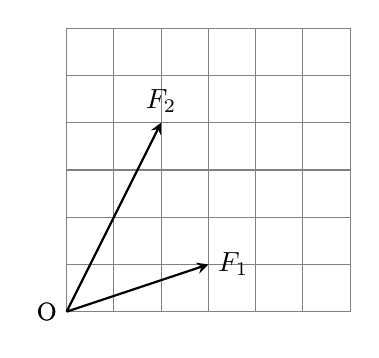
\begin{tikzpicture}[scale = 0.6]
        \foreach \i in {0,...,6}
        {
        \draw[gray](\i,0)to(\i,6);
        }
        \foreach \i in {0,...,6}
        {
        \draw[gray](0,\i)to(6,\i);
        }
        \draw(0,0)node[left]{\small{O}};
        \coordinate[label = left:{\small{O}}](O)at(0,0);
        \coordinate[label = right:$F_1$](F1)at(3,1);
        \coordinate[label = above:$F_2$](F2)at(2,4);
        % 分力
        \draw[thick,-stealth](O)to(F1);
        \draw[thick,-stealth](O)to(F2);
    \end{tikzpicture}
    
    \end{minipage}&
    \begin{minipage}{6cm}
    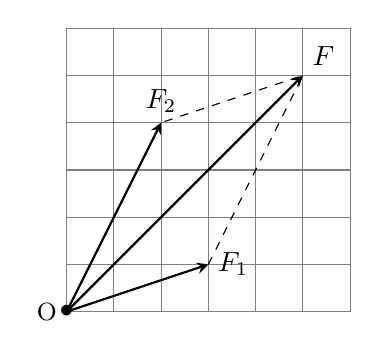
\begin{tikzpicture}[scale = 0.6]
        \foreach \i in {0,...,6}
        {
        \draw[gray](\i,0)to(\i,6);
        }
        \foreach \i in {0,...,6}
        {
        \draw[gray](0,\i)to(6,\i);
        }
        \coordinate[label = left:{\small{O}}](O)at(0,0);
        \coordinate[label = right:$F_1$](F1)at(3,1);
        \coordinate[label = above:$F_2$](F2)at(2,4);
        \coordinate[label = above right:$F$](F)at($(F1)+(F2)$);
        % 合力
        \draw[thick,-stealth](O)node{$\bullet$}to(F);
        % 分力
        \draw[thick,-stealth](O)to(F1);
        \draw[thick,-stealth](O)to(F2);
        % 補助線
        \path[draw, dashed](F1)to(F)to(F2);
    \end{tikzpicture}
    \end{minipage}
    \end{tabular}
\end{center}
合力はこれらを合わせたものだから, 右に$3 + 2 = 5$, 上に$1 + 4 = 5$だけ進むと考えて図を書くと, 平行四辺形の対角線に合力が現れることが分かります.
\begin{exbox}{力の図示の例}
    \begin{center}
    \begin{tabular}{cc}
    \begin{minipage}{6cm}
    物体を斜め上に大きさ$F$の力で引っ張り, 滑らかな水平面上を水平に動かす際の, 重力$W$, 垂直抗力$N$と, $F$の鉛直方向, 水平方向への分力$F_{1}$, $F_{2}$.
    \begin{center}
    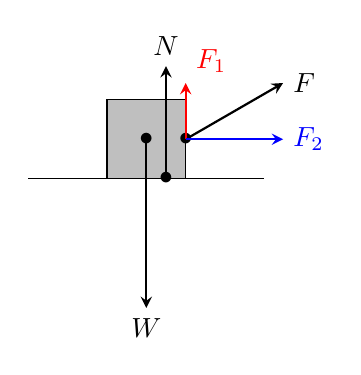
\begin{tikzpicture}[scale = 0.5]
        \path[draw, fill = lightgray](0,0)rectangle(2,2);
        \draw(-2,0)to(4,0);
        \draw[-stealth,thick](2,1)node{$\bullet$}to++(30:20/7)node[right]{$F$}; 
        \draw[-stealth,thick,red](2,1)to++(90:10/7)node[above right]{$F_{1}$}; %鉛直成分
        \draw[-stealth,thick,blue](2,1)to({2+sqrt(3)*10/7},1)node[right]{$F_{2}$};
        \draw[-stealth,thick](1,1)node{$\bullet$}to(1,1-3*10/7)node[below]{$W$}; %重力 
        \draw[-stealth,thick](1.5,0)node{$\bullet$}to(1.5,2*10/7)node[above]{$N$}; %垂直抗力
    \end{tikzpicture}
    \end{center}
    \end{minipage}&
    \begin{minipage}{6cm}
    滑らかな斜面上の物体にはたらく重力$W$と, $W$の斜面方向の分力$W_{1}$, 斜面に垂直な方向の分力$W_{2}$, 垂直抗力. 
    \begin{center}
    \begin{tikzpicture}[scale = 0.5]
        \coordinate(O)at(0,0);
        % 球
        \path[draw,fill=lightgray](O)node[above]{$O$} circle(1);
        \draw(O)node{$\bullet$};
        % 斜面
        \draw[domain=-3:2]plot(\x,{-(1/1.732)*\x-2/1.732}); 
        % 補助線
        \draw[dashed,domain=-2.5:2]plot(\x,{1.732*\x});
        \draw[dashed,domain=-2:2.7]plot(\x,{-1/1.732*\x});
        %重力
        \draw[-stealth,thick](0,0)node{$\bullet$}to(0,-30/7)node[below]{$W$};  
        %垂直抗力
        \draw[-stealth,thick, orange](0,0)++(-120:1)node{$\bullet$}to ++(60:15*1.732/7)node[above right]{垂直抗力};
        % 重力の分力
        \draw[-stealth,thick](0,0)node{$\bullet$}to++(-30:15/7)node[above right]{$W_{1}$};
        \draw[-stealth,thick](0,0)node{$\bullet$}to++(-120:15*1.732/7)node[below left]{$W_{2}$};
    \end{tikzpicture}
    \end{center}
    \end{minipage}
    \end{tabular}
    \end{center}
\end{exbox}
\textbf{球の中心を$O$としたとき, 斜面の斜度は$\angle W O W_{2}$に現れることが, 簡単な考察で分かります}\footnote{保存力の性質から導くことも可能です.}. これは中学生でもできると思いますから, 取り組んでみてください. 

尚, 三角関数を知っている場合, 斜面の斜度を$\theta$として, $W_{1} = W\sin{\theta}$, $W_{2} = W\cos{\theta}$と表せることが分かると思います.

\subsection{瞬間の速度と微分}\label{瞬間の速さと微分}
ここでは, 瞬間の速度について, 微分と絡めて解説してみようと思います. 微分と聞くと難しそうに感じますが, 思ったよりも単純です. ビビらずに進んでみてください. 

時刻$t_0$ [s]から$t_{1}$ [s]の間に, 物体の位置が$x(t_{0})$ [m]から$x(t_{1})$ [m]まで変わったとします. このとき, 時刻$t_{0}$から$t_{1}$間での物体の平均の速度を$v$ [m/s]とすると, 
\begin{equation}
    v = \frac{x(t_{1}) - x(t_{0})}{t_{1} - t_{0}} \label{微分の説明}
\end{equation}
と表されますが, $t_{1} - t_{0}$の間隔を小さくすれば, その速度は, より瞬間の速度を表すことになるでしょう. 具体的には, \textbf{時刻$t_{0}$での瞬間の速度を求めたければ, $t_{1}$を($t_{0}$と一致しないように), $t_{0}$に限りなく近づけたときの$v$の値を求めれば良い} ということです. これは図に起こすと特徴的です. 
時刻$0$から$t$において, 物体が上のような位置の変化で運動したとします. このような時刻と位置をグラフにしたものを, $x$-$t$グラフといいます. 
\begin{center}
    \begin{tabular}{cc}
        \begin{minipage}{7cm}
        \begin{tikzpicture}[scale=0.4]
            % axis
            \coordinate[label=below left:O](O)at(0,0);
            \coordinate[label=right:{時間 $t$ [s]}](t)at(10,0);
            \coordinate[label=above:{位置 $x$ [m]}](x)at(0,8);
            \path[draw, -stealth](-1,0)to(t);
            \path[draw, -stealth](0,-1)to(x);
            % position
            \path[draw, thick, name path=C1]plot[domain = 0:9.5]({\x},{0.1*\x*\x})node[above]{$x(t)$};
            % function
            \path[draw, name path=C2]plot[domain = 2:10]({\x}, {1.2*\x-3.2});
            % calculation of intersections
            \path[name intersections={of=C1 and C2}];
            % coordinates of P
            \coordinate[label=P](P)at(intersection-1);
            \coordinate[label= below:$t_{0}$](T0)at($(O)!(P)!(t)$);
            \coordinate[label= left:$x(t_{0})$](X0)at($(O)!(P)!(x)$);
            \path[draw, dashed](T0)to(P)to(X0);
            % coordinates of Q
            \coordinate[label=Q](Q)at(intersection-2);
            \coordinate[label= below:$t_{1}$](T1)at($(O)!(Q)!(t)$);
            \coordinate[label= left:$x(t_{1})$](X1)at($(O)!(Q)!(x)$);
            \path[draw, dashed](T1)to(Q)to(X1);
        \end{tikzpicture}
        \end{minipage}&
        \begin{minipage}{7cm}
        \begin{tikzpicture}[scale=0.4]
            %axis
            \coordinate[label=below left:O](O)at(0,0);
            \coordinate[label=right:{時間 $t$ [s]}](t)at(10,0);
            \coordinate[label=above:{位置 $x$ [m]}](x)at(0,8);
            \path[draw, -stealth](-1,0)to(t);
            \path[draw, -stealth](0,-1)to(x);
            % function
            \path[draw, name path = C1, thick]plot[domain = 0:8.5]({\x},{0.1*\x*\x});
            % tangent line ちょっとずらしてある.
            \path[draw, name path = C2]plot[domain = 1:9]({\x},{0.8*(\x-4)+1.6});
            % calculation of intersections
            \path[name intersections={of=C1 and C2}];
            % coordinates of P
            \coordinate[label=P](P)at(intersection-1);
            \coordinate[label= below:$t_{0}$](T0)at($(O)!(P)!(t)$);
            \coordinate[label= left:$x(t_{0})$](X0)at($(O)!(P)!(x)$);
            \path[draw, dashed](T0)to(P)to(X0);
        \end{tikzpicture}
        \end{minipage}
    \end{tabular}
\end{center}
\eqref{微分の説明}式は, $x$-$t$グラフ上で「2点P, Qを結んだ直線の傾き」を表していることが分かります. よって, $t_{1}$の値を$t_{0}$に限りなく近づけたとき, \eqref{微分の説明}式は「点Pでのグラフへの接線の傾き」を表していると考えられます. \textbf{よって, 瞬間の速度は, 位置と時刻の関係のグラフにおいて, 「そのグラフへの接線の傾き」として現れてきます}.
\begin{freebox}{関数のグラフと微分}
    一般の関数$f(x)$のグラフでも, $x$の値を, $x=a$に非常に近づけた際の変化の割合$\frac{f(x) - f(a)}{x-a}$は, $f(x)$のグラフに$x = a$で引いた接線の傾きを表すと考えられます. このように, 関数$f(x)$のグラフの$(a, f(a))$で引いた接線の傾きを求めることを, 関数$f(x)$を$x = a$で微分するといいます. 
    \begin{center}
    \begin{tikzpicture}[scale = 0.3]
    \path[draw, domain=-5:6,smooth,thick, name path=C1] plot (\x,{0.1*\x*\x*\x -0.1*\x*\x2 -2*\x})node[right]{$f(x)$};
    \path[draw, domain=-6:-2, name path = C2]plot (\x, {(19/7)*(\x+2.69)+37/10})node[above]{$x=a$での接線};
    \path[name intersections={of = C1 and C2}];
    \coordinate[label=left:{$(a, f(a))$}](P)at(intersection-1);
\end{tikzpicture}
\end{center}
\end{freebox}
これらの考察より, \textbf{物体の位置を時間で微分すると速度になる}と表現できます. また, \eqref{加速度}式より, \textbf{瞬間の加速度は, 速度を時間で微分したものである}といえます. 

\section{運動の法則}
物体の運動において成り立っている性質について, 体系的にまとめ上げた人物がアイザック・ニュートンであり, 微積分学のアイデアを考案した人物の一人としても名高い\footnote{微分, 積分といったアイデアは, アイザック・ニュートンと, ゴットフリート・ライプニッツという人物が, それぞれ独立に考案したと言われており, 現在の微積分学でも, ライプニッツが当時用いていた記号が用いられています. 当時, 必要であった極限, 関数の連続性といった概念はあまり整備されておらず, 現在の数学にも用いられるような厳密な定義は, コーシーや, ワイエルシュトラウスといった数学者たちによって与えられました. }です. 彼は次のような法則を発見しました. \textbf{力学の基礎となる最も重要な法則です}.
\begin{freebox}{ニュートンの運動の法則}
    \begin{enumerate}
        \item \textbf{慣性の法則}：物体に力が働かない場合(物体に働く力の合力が0 Nの場合も含む), 静止している物体は静止し続け, 動いている物体は等速直線運動をする．
        \item \textbf{運動方程式}：物体の受ける合力の大きさ$F$ [N] は, 物体の加速度$a$ [m/s$^2$]と質量$m$ [kg] の積に等しい. 即ち, 
        \begin{equation}
            \bm{F} = \bm{ma} \label{運動方程式}
        \end{equation}
        が成り立つ(本来この式は, 力や加速度の向きを含んで成立する).
        \item \textbf{作用, 反作用の法則}：物体Bが物体Aに力を及ぼすと, 物体Aは物体Bに同じ大きさで反対向きの力を及ぼす. 作用と反作用の力は，同じ作用線上で，反対向きになる．
    \end{enumerate}
\end{freebox}
慣性という言葉が出てきましたが, 物体の慣性とは次のような性質を指します.
\begin{freebox}{慣性}
    物体は, 物体は現在の運動の状態を保っていたいという性質を持っており, この性質を\textbf{慣性}という.
\end{freebox}
慣性はどの物体も持っており, 身近に感じられるものだと思います. これをきっかけに, 普段起きている現象がなぜ, どのようにして起こっているかを考えてみてほしいと思います.
\begin{exbox}{慣性が現れる現象の例}
   \begin{itemize}
    \item 食器が乗ったテーブルのテーブルクロスを素早く引いたとき, 食器が動かずにその場に残るのは, 静止する物体は静止を続けるという物体の慣性が理由です.
    \item 車や自転車, 電車等の乗り物に乗っていて, ブレーキがかかると, 体は前に投げ出されますが, これも, 「もともと前に進んでいたため, そのまま前に進んでいたい」という慣性が原因です.
    \item 宇宙空間でボールを投げると, ボールは投げられた後, 何も力がはたらいていないにも関わらず, 永遠に, 真っ直ぐ同じ速さで進み続けます. これはもともとの運動を保とうとする物体の慣性が現れた結果です.
\end{itemize} 
\end{exbox}

ニュートンの運動の法則それぞれに関して, 説明を加えてみます. 
    \begin{enumerate}
        \item \textbf{慣性の法則}：物体が持つ慣性が現れた結果と見ることができます. 
        \begin{itemize}
            \item 水平な床に置いたペットボトルは, 何も力を加えなければ動くことはありません. 
            \item 例えば, 宇宙空間でボールを投げると, ボールは投げられた後, 何も力がはたらいていないにも関わらず, 永遠に, 真っ直ぐ同じ速さで進み続けます\footnote{厳密には, 地球や他の惑星との万有引力がはたらいており, 多少の加速は生じてしまいますが.}. 
            \item 空気抵抗がなく, なめらかな氷上に置かれた物体は, 一度動かせば止まらず, 永遠に等速でまっすぐ動き続けます. 水平方向には力がはたらいておらず, 重力と垂直抗力がつり合っているため, 実質物体に力がはたらいていないからです.
        \end{itemize}
        \item \textbf{運動方程式}：「物体に力がはたらいている $\Longleftrightarrow$ 物体の運動に加(減)速が生じる」ということを言っています. 
        \begin{itemize}
            \item \eqref{運動方程式} 式より, $F$が一定の値なら($m$：物体の質量の値も一定のため), 加速度$a$も一定の値になります. つまり, 「物体に一定の力がはたらく」$\Longleftrightarrow$「物体の速度が一定の割合で増加(減少)していく」ことが分かります.
        \end{itemize}
        \item \textbf{作用, 反作用の法則}：例を多く挙げることで実感してもらおうと思います. 
        \begin{itemize}
            \item 物体が床から受ける垂直抗力は, 物体が床を押した結果, 床が物体を押し返す力ということができます. 作用, 反作用の法則より, 垂直抗力は, 物体が床を押す力と一直線上にあり, 同じ大きさで, 向きが反対となることが分かります. 
            \item 水泳のターンで, 足で壁を蹴ると前に進みます. 足が壁を後ろ向きに押すと, 作用・反作用の法則により, 壁から足には前向きに同じ大きさの力がはたらきます. この力によって体が前向きに加速されるため, 前へ進みます\footnote{自分が加えた力の向きと, 自分が動く向きが反対になっていることを考えると, 少し不思議な感じがするかもしれません. }.
            \item 消しゴムで文字を消していたら, 紙がぐしゃっとなってしまうことがあると思います. 簡単のため, 紙面の上側を手で抑え, 消しゴムを動かす方向を紙面上向きとしてみます. 消しゴムにかかる摩擦力は, 動かす方向と反対となるため紙面下向きです. このとき作用, 反作用の法則により, 紙は, 紙面上向きで, 消しゴムにかかる摩擦力と一直線上にあり, 同じ大きさの力を受けます. その結果紙は抑えている手の方に寄ってしまうため, 場合によってはグシャッとなってしまいます. 
        \end{itemize} 
    \end{enumerate}
\subsection{つり合いと作用, 反作用}
「力がつり合っている」とはどういうことでしょうか. これは次のように表現できます.
\begin{freebox}{力のつり合い}
    \textbf{1つの物体に複数の力がはたらいていて, 物体にはたらく合力が0になるとき, それらの力はつり合っているという}.
\end{freebox}
ここで, 少し運動の法則について考察を行います. 
\begin{itemize}
    \item 慣性の法則から, 物体に力が実質はたらいていないとき, 物体は等速直線運動, または静止することが分かります.
    \item 逆に, 物体が等速直線運動している, または静止しているとき, \eqref{運動方程式} 式において$a=0$のため, $F = 0$を得ます. つまり, 物体が静止または等速直線運動しているならば, 物体にはたらく力はすべてつり合っているということです.
\end{itemize}
よって次を結論できます.
\begin{freebox}{静止とつり合い}
「物体が静止または等速直線運動していること」と「各物体にはたらく力がすべてつり合っていること」は\textbf{同じである}.
\end{freebox}
ところで, つり合っている2力は, 
\begin{itemize}
    \item 向きが反対である.
    \item 力の大きさが等しい.
    \item 一直線上にある.
\end{itemize}
という条件を満たします. また, 作用, 反作用による力も, 上の条件を満たします. それでは「つり合い」「作用, 反作用」の違いは何でしょうか. \textbf{前者は「1つの物体にはたらく力たちの関係」であり, 後者は「2つの物体の間にはたらく力の関係」という違いがあります}. 
 
\begin{exbox}{つり合いと作用, 反作用}
    \textbf{\ref{力の図示} 節の$(\ast)$を思い出しましょう}.
    \begin{itemize}
    \item 天井に軽いばねを固定し, ばねに物体をつけて静止させたとき,
    \begin{center}
    \begin{tabular}{cc}
    \begin{minipage}{5cm}
    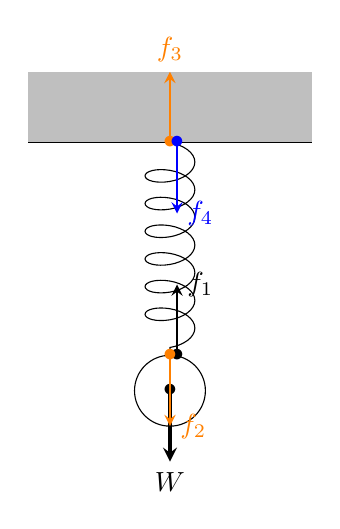
\begin{tikzpicture}[scale = 0.9]
        \coordinate(V1)at(0,1);
        \coordinate(O)at(0,0);
        \coordinate(W1)at(0,-0.5);
        \coordinate(F1)at(0.1,0);
        \coordinate(F3)at(0,3);
        \coordinate(F4)at(0.1,3);
        \fill[lightgray](-2,4) rectangle(2,3);
        \path[draw](-2,3)to(2,3);
        \draw[decorate,decoration={coil,amplitude=9pt}] (0,3) to (O);
        \draw (W1) circle(0.5);
        % force
        % sphere
        \path[draw, very thick, -stealth](W1)node{$\bullet$}to($(W1)-(V1)$)node[below]{$W$}; 
        \path[draw, thick, -stealth](F1)node{$\bullet$}to($(F1)+(V1)$)node[right]{$f_{1}$};
        % ばね
        \path[draw, thick, -stealth, orange](O)node{$\bullet$}to($(O)-(V1)$)node[right]{$f_{2}$};
        \path[draw, thick, -stealth, orange](F3)node{$\bullet$}to($(F3)+(V1)$)node[above]{$f_{3}$};
        % 天井
        \path[draw, thick, -stealth, blue](F4)node{$\bullet$}to($(F4)-(V1)$)node[right]{$f_{4}$};
    \end{tikzpicture}
    \end{minipage}&
    \begin{minipage}{6cm}
    \begin{itemize}
        \item $W$：物体にはたらく重力
        \item $f_{1}$：ばねが物体を引く力
        \item $f_{2}$：物体がばねを引く力
        \item $f_{3}$：天井がばねを引く力
        \item $f_{4}$：ばねが天井を引く力
    \end{itemize}
    $W$, $f_{1}$が物体にはたらく力で, $f_{2}, f_{3}$がばねにはたらく力, $f_{4}$が天井にはたらく力です. 本来はばねにも重力がかかりますが, 軽いため無視できます.
    \begin{itemize}
        \item \textbf{つり合いの関係の力}：$W$と$f_{1}$, $f_{2}$と$f_{3}$ .
        \item \textbf{作用, 反作用の関係の力}：$f_{1}$と$f_{2}$, $f_{3}$と$f_{4}$.
    \end{itemize}
    \end{minipage}
    \end{tabular}     
    \end{center}
    よって, 力の大きさの関係は, $W = f_{1}$, $f_{2}= f_{3}$, $f_{1} = f_{2}$, $f_{3} = f_{4}$. 
    
    つまり, $W = f_{1} = f_{2} = f_{3} = f_{4}$です. 

    \item  物体1, 物体2, 物体3を, その順で下から3つ重ねて静止させたとき(今回, 長さは正確ではありません),
    \begin{center}
    \begin{tabular}{cc}
    \begin{minipage}{5cm}
    \centering
    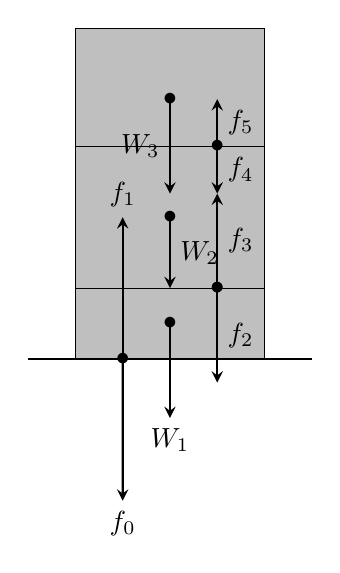
\begin{tikzpicture}[scale = 0.6]
        \coordinate(V1)at(0,1);
        \path[draw](-3,-0.5)to(3,-0.5);
        \coordinate(O1)at(-2,-0.5);
        \coordinate(O2)at(2,1);
        \coordinate(O3)at(-2,4);
        \coordinate(O4)at(2,6.5);
        % gravity
        \coordinate(W1)at($(O1)!0.5!(O2)$);
        \coordinate(W2)at($(O2)!0.5!(O3)$);
        \coordinate(W3)at($(O3)!0.5!(O4)$);
        % resistance?
        \coordinate(F0)at(-1,-0.5);
        \coordinate(F2)at(1,1);
        \coordinate(F4)at(1,4);
        % 下
        \path[draw, fill = lightgray](O1)rectangle(O2);
        % 中
        \path[draw, fill = lightgray](O2)rectangle(O3);
        % 上
        \path[draw, fill = lightgray](O3)rectangle(O4);
        % force
        % 下
        \path[draw, thick, -stealth](W1)node{$\bullet$}to($(W1)-2*(V1)$)node[below] {$W_{1}$}; 
        \path[draw, thick, -stealth](F0)node{$\bullet$}to ($(F0)+3*(V1)$)node[above]{$f_{1}$}; % 3cm
        \path[draw, thick, -stealth](F2)node{$\bullet$}to node[midway, right] {$f_{2}$}($(F2)-2*(V1)$); % 2cm
        % 中
        \path[draw, thick, -stealth](W2)node{$\bullet$}to node[midway, right] {$W_{2}$}($(W2)-1.5*(V1)$);
        \path[draw, thick, -stealth](F2)node{$\bullet$}to node[midway, right] {$f_{3}$}($(F2)+2*(V1)$); 
        \path[draw, thick, -stealth](F4)node{$\bullet$}to node[midway, right] {$f_{4}$}($(F4)-(V1)$); 
        % 上
        \path[draw, thick, -stealth](0,5)node{$\bullet$}to node[midway, left] {$W_{3}$}(0,3);
        \path[draw, thick, -stealth](F4)to node[midway, right] {$f_{5}$}($(F4)+(V1)$); 
        % 床
        \path[draw, thick, -stealth](-1,-0.5)to ($(F0)-3*(V1)$)node[below]{$f_{0}$}; 
    \end{tikzpicture}
    \end{minipage}&
    \begin{minipage}{6cm}
    \begin{itemize}
        \item $W_{1}$：物体1にはたらく重力
        \item $W_{2}$：物体2にはたらく重力
        \item $W_{3}$：物体3にはたらく重力
        \item $f_{0}$：物体1が床を押す力
        \item $f_{1}$：地面が物体1を押す力
        \item $f_{2}$：物体2が物体1を押す力
        \item $f_{3}$：物体1が物体2を押す力
        \item $f_{4}$：物体3が物体2を押す力
        \item $f_{5}$：物体2が物体3を押す力
    \end{itemize}
    \end{minipage}
    \end{tabular}     
    \end{center}
    $W_{1}, f_{1}, f_{2}$が物体1にはたらく力で, $W_{2}, f_{3}, f_{4}$が物体2にはたらく力, $W_{3}, f_{5}$が物体3にはたらく力です. 
    \begin{itemize}
        \item \textbf{つり合いの関係の力}：$W_{1} + f_{2}$と$f_{1}$, $W_{2}+ f_{4}$と$f_{3}$, $W_{3}$と$f_{5}$.
        \item \textbf{作用, 反作用の関係の力}：$f_{0}$と$f_{1}$, $f_{2}$と$f_{3}$, $f_{4}$と$f_{5}$.
    \end{itemize}
    よって, 力の大きさの関係は, $W_{1} + f_{2} = f_{1}$, $W_{2}+ f_{4} = f_{3}$, $W_{3} = f_{5}$, $f_{0} = f_{1}$, $f_{2} = f_{3}$, $f_{4} = f_{5}$. 
    よって例えば, $f_{0} = f_{1} = W_{1} + W_{2} + W_{3}$, $f_{2} = f_{3} = W_{2} + W_{3}$, $f_{4} = f_{5} = W_{3}$が導け, 確かに直感と一致しています. 
    \end{itemize}
\end{exbox}
高校では, 力のつり合い, 作用, 反作用の法則を用いることで, 力たちの関係を式で表現する場面が多くあります.  次のような例を考えてみましょう. 内容自体は中学生が理解可能なレベルですが, 文字式を用いている点が新鮮に感じると思います. 
\begin{exbox}{高校生で習う物理の初歩}
    空気抵抗は無視できるものとし, 重力加速度の大きさを$g$ [m/s$^2$]とします. 質量$M$ [kg]の板が床の上にあって, 板の上に, 質量$m$ [kg] の石が1つ載っており, 全体が静止している状況を考えてみます. \textbf{重力加速度の定義から, 質量$m$ [kg]の物体には$mg$ [N]の重力がかかる}ことに注意しましょう.
        \begin{center}
            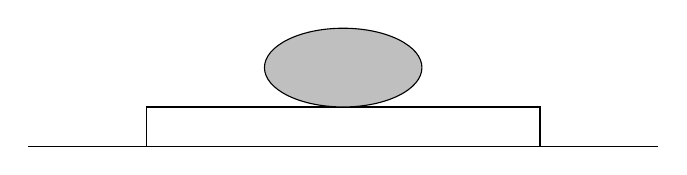
\begin{tikzpicture}[scale = 0.5]
                \path[draw](-3,0) to (13,0);
                \coordinate(A) at (0,0);
                \coordinate(B) at (10,1);
                \path[draw] (A) rectangle(B);
                \path[draw, fill = lightgray](5,2) circle[x radius = 2cm, y radius = 1cm];
            \end{tikzpicture}
        \end{center}
        \begin{enumerate}
            \item 石が板から受ける垂直抗力を$N_{1}$ [N]とすると, $N_{1}$は何Nですか.
            \item 板が床から受ける垂直抗力を$N_{2}$ [N]とすると, $N_{2}$は何Nですか.
        \end{enumerate}
        \textbf{全体は静止しているため, 各物体にはたらく力はつり合っています}. ここでは下向きを正の方向とし, \ref{力の図示} 節の$(\ast)$に注意しながら, 各物体にはたらく力を書いていきます. 作用, 反作用の法則より, 板も石から力を受けていることに注意しましょう. 
        \begin{center}
        \begin{tabular}{cc}
        \begin{minipage}{6cm}
        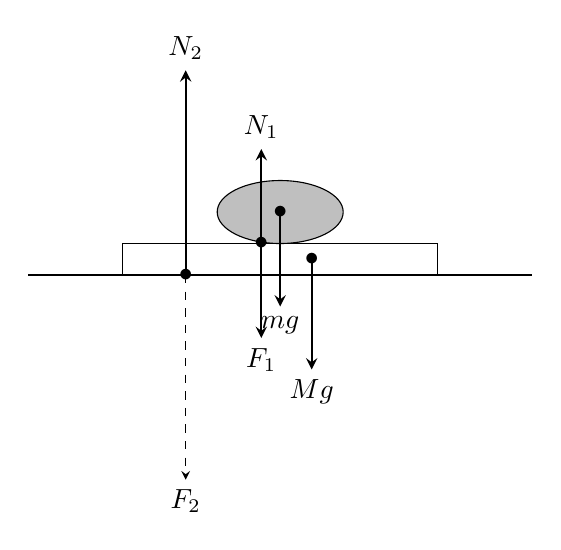
\begin{tikzpicture}[scale=0.4]
            % 床
            \path[draw](-3,0) to (13,0);
            \coordinate(A) at (0,0);
            \coordinate(B) at (10,1);
            % 石
            \path[draw, fill = lightgray](5,2) circle[x radius = 2cm, y radius = 1cm];

            % 石重力 3cm
            \draw[thick,-stealth](5,2)node{$\bullet$}to(5,-1)node[below]{$mg$};

            % 板
            \path[draw] (A) rectangle(B);

            % 板重力 3.5cm
            \draw[thick,-stealth](6,0.5)node{$\bullet$}to(6,-3)node[below]{$Mg$};

            % 石と板の作用反作用
            \path[draw, -stealth, thick](4.4,1)node{$\bullet$}to(4.4,4)node[above]{$N_1$};
            \path[draw, -stealth, thick](4.4,1)to(4.4,-2)node[below]{$F_1$};

            % 板と床の作用反作用
            \path[draw, -stealth, thick](2,0)node{$\bullet$}to(2,6.5)node[above]{$N_2$};
            \path[draw, -stealth, dashed](2,0)to(2,-6.5)node[below]{$F_2$};
        \end{tikzpicture}
        \end{minipage}&
        \begin{minipage}{6cm}
        $F_{1}$は石が板を押す力で, $N_{2}$と作用, 反作用の関係です. 大きさについて$N_{1} = F_{1}$. 各物体にはたらく力の合力が0という式を立てると, 
        \begin{equation}
        \begin{cases}
            石: &  mg - N_{1} = 0\\
            板: &  Mg + F_1 - N_{2} = 0.
        \end{cases}
        \end{equation}
        よって, $N_{1} = mg$ [N], \\
        $N_{2} = (M+m)g$ [N]です. 
        \end{minipage}
        \end{tabular}
        \end{center}
        
        確かに, $N_{2}$が$Mg$ [N]にならないのは直感とも(上に物体が載っているため)一致しているのではないでしょうか. 尚, 点線で書いた$F_{2}$は, 板が床を押す力で, $N_{2}$と作用, 反作用の関係です. しかし, $F_{2}$は床にはたらく力のため, 今回は関係ありません. 
    \end{exbox}

\section{一定の力がはたらく運動}\label{一定の力がはたらく運動}
ニュートンの運動の法則の運動方程式(\eqref{運動方程式} 式)により, \textbf{一定の力がはたらく運動では, 加速度が一定になる}ことが分かりますが, このような運動を, \textbf{等加速度直線運動}といいます. ここでは等加速度直線運動について考察を深めます. まずは例から見てみましょう.
\begin{exbox}{等加速度直線運動の例}
    \begin{itemize}
        \item スキーやスノーボードで斜面を直滑降すると, 斜面上の等加速度直線運動となります. 板と人を一体の物体とみなすと, その物体は, 斜面方向について, 重力の斜面方向の分力と, (動)摩擦力の合力を受けますが, その合力の大きさは一定だからです. 
        \begin{center}
        \begin{tikzpicture}[scale=0.6]
            %球
            \fill[lightgray](0,0)circle(1);
            \draw(0,0)circle(1);
            \draw(0,0)node{$\bullet$};
            %斜面
            \draw[domain=-3:2]plot(\x,{-(1/1.732)*\x-2/1.732}); 
            %補助線
            \draw[dashed,domain=-2.3:1]plot(\x,{1.732*\x});
            \draw[dashed,domain=-2:2.7]plot(\x,{-1/1.732*\x});
            %重力
            \draw[-stealth,thick](0,0)node{$\bullet$}to(0,-30/7)node[below]{重力};  
            %垂直抗力
            \draw[-stealth,thick,orange](0,0)++(-120:1)node{$\bullet$}to ++(60:15*1.732/7)node[above right]{垂直抗力};
            % 重力の分力
            \draw[-stealth,thick](0,0)node{$\bullet$}to++(-30:15/7)node[above right]{重力の斜面に平行な成分};
            \draw[-stealth,thick](0,0)node{$\bullet$}to++(-120:15*1.732/7)node[below left]{重力の斜面に垂直な成分};
            % 摩擦力
            \draw[-stealth,thick,red](0,0)++(-120:1)node{$\bullet$}to ++(150:1)node[left]{摩擦力};
        \end{tikzpicture}
        \end{center}
        \item 自由落下も, (空気抵抗を無視すると)等加速度直線運動です. 自由落下中に, 物体は一定値の重力のみを受けるからです.
        \item 花火が打ち上がる間の運動も, (空気抵抗を無視すると)等加速度直線運動です. 花火が上がる間, 花火の受ける力は一定値の重力のみだからです. 
        
        重力は花火の初速度の方向とは反対のため, 初速度の方向を正とすると, 花火は負の加速度を受け, 最高点に達するまで一定の割合で減速していくことが分かります. 
    \end{itemize}
\end{exbox}
\subsection{等加速度直線運動している物体の速度}\label{等加速度直線運動している物体の速度}
加速度とは, 1秒(単位時間)あたりに増加(減少する)速度のことだったことを思い出しておきましょう. すると, 等加速度直線運動の場合には, 次のようなことが分かります. $t$秒後の速度を$v$ [m/s], 初速度$v_{0}$ [m/s], 加速度の大きさを$a$ [m/s$^2$]\footnote{時間に依存せず一定値であることが分かる.}とします. このとき物体の速度は, 1秒で$a$ [m/s]だけ加速するため, 
\begin{freebox}{$t$秒後の速度}
    初速度の向きを正の向きとする. 等加速度直線運動している物体の, 計測から$t$秒後の速度$v$は, 
    \begin{equation}
        \bm{v} = \bm{v_{0}} + \bm{at} \label{等加速度直線運動-速度}
    \end{equation}
    で与えられる. 
\end{freebox}
\eqref{等加速度直線運動-速度} 式より, 等加速度直線運動では, \textbf{縦軸を速度, 横軸を時刻としてグラフを書くと, 切片が$\bm{v_{0}}$, 傾きが$\bm{a}$となる一次関数が書ける}ということです. 
\begin{freebox}{速度と時刻のグラフ}
    等加速度直線運動について, 速度と時間の関係をグラフで表すと次のようになる. 
    \begin{center}
    \begin{tikzpicture}[scale=0.4]
            % axis
            \coordinate[label=below left:O](O)at(0,0);
            \coordinate[label=right:{時間 $t$ [s]}](t)at(10,0);
            \coordinate[label=above:{速度 $v$ [m/s]}](x)at(0,8);
            \path[draw, -stealth](-1,0)to(t);
            \path[draw, -stealth, name path = X](0,-1)to(x);
            % velocity
            \path[draw, name path=C1, thick]plot[domain = 0:10]({\x}, {0.5*\x+2})node[right]{$v = v_{0} + at$};
            %intersections
            \path[name intersections={of=C1 and X}];
            \coordinate[label=left:$v_{0}$](v0)at(intersection-1);
        \end{tikzpicture}
        \end{center}
        尚, 直線の傾きに加速度が表れる. \ref{加速度とは} 節や, \eqref{加速度} 式も確認せよ.
\end{freebox}

\subsection{等加速度直線運動している物体の移動距離}\label{等加速度直線運動している物体の移動距離}
次に, 物体の移動距離に関しても考察を深めましょう. 「物体の移動距離」という言葉を使っていますが, 正確には「物体の位置」を表しています. \ref{等加速度直線運動している物体の速度} 節の\textbf{速度と時刻のグラフ}\footnote{このようなグラフを$v$-$t$グラフといいます.}について, このグラフを長方形たちに区切ってみます. 一つ一つの長方形の面積は, $「速さ」\times「経過時間」$を表しているため, 区切った時間で移動した距離を表すはずです. 
\begin{center}
\begin{tabular}{cc}
    長方形に分割 & 長方形の分割を細かくする\\
    \begin{minipage}{7cm}
    \begin{center}
    \begin{tikzpicture}[scale=0.37]
        % axis
        \coordinate[label=below left:O](O)at(0,0);
        \coordinate[label=right:{時間 $t$ [s]}](t)at(10,0);
        \coordinate[label=above:{速度 $v$ [m/s]}](x)at(0,8);
        \path[draw, -stealth](-1,0)to(t);
        \path[draw, -stealth, name path = X](0,-1)to(x);
        % velocity
        \path[draw, name path=C1]plot[domain = 0:10]({\x}, {0.5*\x+2})node[right]{$v = v_{0} + at$};
        %intersections
        \path[name intersections={of=C1 and X}];
        \coordinate[label=left:$v_{0}$](v0)at(intersection-1);
        % 区分求積
        \foreach \x in {0,1,2,...,8}
        {
            \path[draw, fill = lightgray](\x,0)to(\x,{0.5*\x+2})to(\x+1,{0.5*\x+2})to(\x+1,0)--cycle; 
        }  
    \end{tikzpicture}
    \end{center}
    \end{minipage}&
    \begin{minipage}{7cm}
    \begin{center}
    \begin{tikzpicture}[scale=0.37]
        % axis
        \coordinate[label=below left:O](O)at(0,0);
        \coordinate[label=right:{時間 $t$ [s]}](t)at(10,0);
        \coordinate[label=above:{速度 $v$ [m/s]}](x)at(0,8);
        \path[draw, -stealth](-1,0)to(t);
        \path[draw, -stealth, name path = X](0,-1)to(x);
        % velocity
        \path[draw, name path=C1]plot[domain = 0:10]({\x}, {0.5*\x+2})node[right]{$v = v_{0} + at$};
        %intersections
        \path[name intersections={of=C1 and X}];
        \coordinate[label=left:$v_{0}$](v0)at(intersection-1);
        %区分求積
        \foreach \x in {0,1,2,...,44}
        {
            \path[draw,fill=lightgray]({\x/5},0)to({\x/5},{0.5*(\x/5)+2})to({(\x+1)/5},{0.5*(\x/5)+2})to({(\x+1)/5},0)--cycle;
        }
    \end{tikzpicture}
    \end{center}
    \end{minipage}
    \end{tabular}
\end{center}
よって, \textbf{この長方形の面積和は, 物体の総移動距離を表している}ことが分かります. よって, 長方形の分割を限りなく小さくすれば\footnote{つまり, 時間をものすごく細かく区切れば}, その面積の和は正確な総移動距離を表すことになるでしょう. つまり, \textbf{グラフと時間軸で囲まれた部分の面積を求めれば, 物体の総移動距離を求めることができるということです}. $t$秒後であれば, 底辺$t$, 高さ$v_{0}$の下の長方形と, 底辺$t$, 高さ$at$の三角形の面積の合計を考えることにより, 次が分かります.
\begin{freebox}{$t$秒後の移動距離}
    初速度の方向を正とする. 初速度$v_{0}$ [m/s],一定加速度$a$ [m/s$^2$]で等加速度直線運動している物体の物体の, 計測から$t$秒後の移動距離は, 
    \begin{equation}
        \bm{x} = \bm{v_{0}t} + \bm{\frac{1}{2}at^2} \label{等加速度直線運動-位置}
    \end{equation}
    である. \textbf{つまり, 物体の移動距離は, 時刻の2次関数となることが分かる}. 
\end{freebox}
実は, \ref{瞬間の速さと微分} 節の$x$-$t$グラフは, 初速度$v_{0} = 0$の等加速度直線運動のものです.
有名な事実かもしれませんが, \eqref{等加速度直線運動-速度} 式や, \eqref{等加速度直線運動-位置} 式を見て分かるように, 物体の速度と位置に, 物体の質量は関係していません. よって, 次のような例があります.
\begin{exbox}{直感に反する例}
    空気抵抗がない状態で, 鉄球とアリを, 同じ高さから手を離すことで自由落下させます. このとき, 鉄球もアリも, 全く同じタイミングで地面に着きます. また, ストロボ写真をとっても, 全く同じ動きの写真が撮れます.
\end{exbox}
普段は重いものほど早く落ちますが, 空気抵抗がない場合,\textbf{「重いものほど早く落ちる」という直感が否定される}ことになります. 
\begin{freebox}{関数のグラフと積分}
    \begin{center}
    \begin{tabular}{cc}
    \begin{minipage}{6cm}
    \centering
    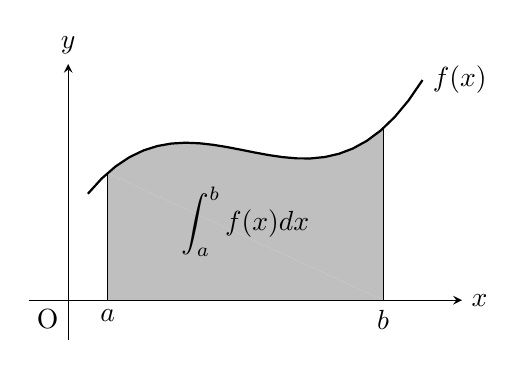
\begin{tikzpicture}[scale = 0.5]
        % points
        \coordinate[label = below:$a$](A)at(1,0);
        \coordinate[label = below:$b$](B)at(8,0);
        % fill
        \path[fill = lightgray]plot[domain = 1:8](\x,{(4/135)*(\x)^3-(2/5)*(\x)^2+(8/5)*\x+2})to (B);
        \path[fill = lightgray](A)to(1,{4/135-2/5+8/5+2})to (B) to cycle;
        % graph
        \path[draw,thick]plot[domain = 0.5:9](\x,{(4/135)*(\x)^3-(2/5)*(\x)^2+(8/5)*\x+2})node[right]{$f(x)$};
        % axis
        \coordinate[label=below left:O](O)at(0,0);
        \coordinate[label=right:$x$ ](x)at(10,0);
        \coordinate[label=above:$y$](y)at(0,6);
        \path[draw, -stealth, name path = X](-1,0)to(x);
        \path[draw, -stealth](0,-1)to(y);
        \path[draw](A)to (1,{4/135-2/5+8/5+2});
        \path[draw](B)to (8,{(4/135)*8^3-(2/5)*8^2+(8/5)*8+2});
        % integral
        \draw(4.5,2)node{$\displaystyle \int_{a}^{b}f(x)dx$};
    \end{tikzpicture}
    \end{minipage}&
    \begin{minipage}{6cm}
    前の議論のように, 関数$f(x)$のグラフと$x= a$, $x = b$で囲まれた部分の面積を求めることを, 関数$f(x)$を$x = a$から$x = b$まで積分するという.
    \begin{equation}
        数式では,\ \int_{a}^{b}f(x)dx\ と書く.
    \end{equation} 
    \end{minipage}
    \end{tabular}
    \end{center}
    積分を知っているなら, $\int_{0}^{t}v(t)dt = \int_{0}^{t} (v_{0} + at) dt$を計算すれば\eqref{等加速度直線運動-位置} 式を導ける.
\end{freebox}
ところで, \eqref{等加速度直線運動-速度}, \eqref{等加速度直線運動-位置} 式だけでは, 時刻$t$での速度, 位置の関係を直接見ることができません. 速度と位置の関係式を導出することを考えてみます. \eqref{等加速度直線運動-速度} 式から, $t = \frac{v - v_{0}}{a}$と表せるため, この$t$を\eqref{等加速度直線運動-位置} 式に代入することで次の式を得ます. \textbf{実際に計算し, これが成立することを各自で必ず確認してください}.
\begin{freebox}{速度と位置の関係}
加速度$a$ [m/s$^2$] で等加速度直線運動する物体について, 時間を固定した際の位置, 速度の関係は以下である.
\begin{equation}
    \bm{v^2} - \bm{v_{0}^2} = \bm{2ax} \label{速度と位置の関係}
\end{equation}
\end{freebox}
この式により, 時間を固定した際の速度, 加速度, 位置の関係がひと目で分かります. 
 
\section{力がはたらかない運動}\label{力がはたらかない運動}
このとき, 慣性の法則が成り立ちます. つまり, 物体は静止していれば静止を続け, 運動していたとしても, それは等速直線運動となります. 
\begin{exbox}{等速直線運動の例}
雨粒が雲から地面に落ちてくる際, 途中で空気抵抗と重力がつり合い, 雨粒にはたらく合力が0になります. よって, 雨粒はその間等速直線運動します. 

地上5000mから降った雨粒が, もし空気抵抗を受けずに自由落下すると, 重力加速度を約10m/s$^2$として\eqref{速度と位置の関係}式から計算すれば, 雨粒の速さは約316m/sとなって, ものすごい速さになってしまいます. ちなみに音速が約340m/sです.
\end{exbox}
動いている物体について, 多くの人が陥りやすい勘違いとして, 
\begin{quotation}
    物体が運動しているならば, 物体に力がはたらいている
\end{quotation}
というものがあります. \textbf{これは誤りです}. 
実際, 
\begin{exbox}{運動しているが力がはたらいていない例}
    宇宙空間でボールを投げると, ボールは投げられた後, 何も力がはたらいていないにも関わらず, 永遠に, 真っ直ぐ同じ速さで進み続けます(慣性による). 
\end{exbox}
改めて正しい解釈を述べておきます. 
\begin{freebox}{運動と力}
    \begin{itemize}
        \item \textbf{物体に力がはたらいていて, はたらく力の合力が0でない}$\Longleftrightarrow$ \textbf{物体に加(減)速が生じる}
        \item \textbf{物体に力は実質はたらいてない(つり合っている場合を含む)}
        $\Longleftrightarrow$
        \textbf{物体に加(減)速が生じない}
        $\Longleftrightarrow$ \textbf{物体が等速直線運動する(静止も含む)}
    \end{itemize}
\end{freebox}
よって, 等速直線運動している物体については, \eqref{等加速度直線運動-速度}, \eqref{等加速度直線運動-位置} 式において, 加速度$a=0$としたものを考えれば良く, 次の関係式を得られます. 速度が一定なため当たり前に思えるのではないでしょうか. 
 
\begin{freebox}{等速直線運動している物体の速度と移動距離}
初速度の向きを正とする. 初速度$v_{0}$ [m/s]で等速直線運動している物体の, 計測から$t$秒後の速度$v$ [m/s]と, 移動距離$x$ [m]は以下で与えられる.
\begin{align}
    \bm{v} &= \bm{v_{0}}, \label{等速直線運動-位置}\\
    \bm{x} &= \bm{v_{0}t}. \label{等速直線運動-位置}
\end{align}
\end{freebox}
よって, $x$-$t$グラフ, $v$-$t$グラフは次のようになります.
\begin{freebox}{等速直線運動とグラフ}
\begin{center}
\begin{tabular}{cc}
\begin{minipage}{6cm}
\begin{tikzpicture}[scale=0.4]
    % axis
    \coordinate[label=below left:O](O)at(0,0);
    \coordinate[label=right:{時間 $t$ [s]}](t)at(10,0);
    \coordinate[label=above:{速度 $v$ [m/s]}](x)at(0,8);
    \path[draw, -stealth](-1,0)to(t);
    \path[draw, -stealth, name path = X](0,-1)to(x);
    % velocity
    \path[draw, name path=C1, thick]plot[domain = 0:8]({\x}, 6)node[right]{$v = v_{0}$};
    %intersections
    \path[name intersections={of=C1 and X}];
    \coordinate[label=left:$v_{0}$](v0)at(intersection-1);
\end{tikzpicture}
\end{minipage}&
\begin{minipage}{6cm}
\begin{tikzpicture}[scale=0.4]
    % axis
    \coordinate[label=below left:O](O)at(0,0);
    \coordinate[label=right:{時間 $t$ [s]}](t)at(10,0);
    \coordinate[label=above:{移動距離 $x$ [m]}](x)at(0,8);
    \path[draw, -stealth](-1,0)to(t);
    \path[draw, -stealth, name path = X](0,-1)to(x);
    % velocity
    \path[draw, thick]plot[domain = 0:8]({\x}, {\x})node[right]{$x = v_{0}t$}to(O);
\end{tikzpicture}
\end{minipage}
\end{tabular}
\end{center}
$v-t$グラフと時間軸で囲まれた部分の面積は, \ref{等加速度直線運動している物体の移動距離} 節で解説したように, 物体の移動距離を表しており, $t$秒後においては確かに$v_{0}t$となっています.
\end{freebox}
\section{\ref{一定の力がはたらく運動}, \ref{力がはたらかない運動} 章の応用例}
物体を地面から斜めに発射すると, 上に凸の放物線を描いて運動することは有名でしょう. 実は, これまでの知識を用いることで, 軌道が放物線となることを説明できます. 空気抵抗は無視するとして考えてみましょう. 
\begin{center}
    \begin{tikzpicture}[scale=1.2]
        \coordinate[label = left:O](O)at(0,0);
        \coordinate[label = right:$x$](x)at(8,0);
        \coordinate[label = $y$](y)at(0,3);
        % axis
        \path[draw,-stealth](O)to(x);
        \path[draw,-stealth](O)to(y);
        % graph
        \path[draw]plot[domain = 0:6](\x, {-0.3*\x*\x+1.8*\x});
        % v0
        \coordinate[label = right:$v_{0}$](P)at(1,{sqrt(3)});
        \coordinate[label = below:$v_{0_{x}}$](Q)at(1,0);
        \coordinate[label = above left:$v_{0_{y}}$](R)at(0,{sqrt(3)});
        \coordinate[label = above right:$\theta$](S)at(0.2,0.05);
        \path[draw, -stealth](O)to(Q);
        \path[draw, -stealth](O)to(R);
        \path[draw, -stealth, thick](O)to(P);
        \path[draw, dashed](O)rectangle(P);
        \path pic[draw,angle radius=3mm] {angle=Q--O--P};
    \end{tikzpicture}
\end{center}
複雑なものは分けるという発想で. 今回は物体の運動を水平($x$)方向と鉛直($y$)方向に分解してみます. 初速度$v_{0}$の$x$方向の成分を$v_{0_{x}}$, $y$方向の成分を$v_{0_{y}}$と書くことにします. 運動中に物体が受ける力は, 各方向で次のようになります.
\begin{itemize}
    \item 鉛直方向では, 重力のみがはたらく. 
    \item 水平方向には, 何も力がはたらいていない. つまり水平方向には等速直線運動する. 
\end{itemize}
よって, 運動の様子は
\begin{itemize}
    \item 鉛直方向では, 上に上がってから, 落ちてくる運動
    \item 水平方向には, 一定速度で一直線に進む運動
\end{itemize}
となります. これらが同時に起こっているため, 軌道は上に凸の放物線になることが, 直感的にも分かるのではないでしょうか. 式を用いて説明すると, 次のようになります. 
\begin{freebox}{式を用いた説明}
初速度$v_{0}$で斜めに発射することを考えます. 各方向では, 初速度の成分の向き正とします. 鉛直方向の運動方程式は, 物体の質量を$m$として, 
\begin{equation}
    ma = -mg. \quad a = -g
\end{equation}
つまり物体の加速度は, 鉛直方向の初速度と反対向きに, 一定の$g$ [m/s$^2$]であることが分かります. これと\eqref{等加速度直線運動-位置} 式より, $t$秒後での鉛直方向の位置$y$は, 次のようになります.
\begin{equation}
    y = v_{0_{y}}t -\frac{1}{2}gt^2.\label{斜方投射の応用-鉛直方向の位置}
\end{equation}
一方, $t$秒後での水平方向の位置$x(t)$は, 速度$v_{0_{x}}$ [m/s]での等速直線運動を考えて
\begin{equation}
    x = v_{0_{x}}t\label{斜方投射の応用-水平方向の位置}
\end{equation}
です. \eqref{斜方投射の応用-水平方向の位置} 式を$t$について解くと, $t = x/v_{0_{x}}$であり, これを\eqref{斜方投射の応用-鉛直方向の位置} 式に代入すると, 
\begin{align}
    y = v_{0_{y}}t -\frac{1}{2}gt^2
    = \frac{xv_{0_{y}}}{v_{0_{x}}} - \frac{1}{2}g\left(\frac{x}{v_{0_{x}}}\right)^2
    = -\frac{g}{2v_{0_{x}}^2}x^2 + \frac{v_{0_{y}}}{v_{0_{x}}}x.
\end{align}
つまり, $y$は$x$の, $2$次の係数が負の2次関数として書かれ, \textbf{軌道は上に凸の放物線になることが分かります}. 尚, 直前に求めた$y$を平方完成すると, 
\begin{align}
    y &=  -\frac{g}{2v_{0_{x}}^2}x^2 + \frac{v_{0_{y}}}{v_{0_{x}}}x = -\frac{g}{2v_{0_{x}}^2}\left(x - \frac{v_{0_{x}}v_{0_{y}}}{g}\right)^2 + \frac{v_{0_{y}}^2}{2g}
\end{align}
となるため, (高校生なら)軸が$x = \frac{v_{0_{x}}v_{0_{y}}}{g}$, 頂点の座標が$\left(\frac{v_{0_{x}}v_{0_{y}}}{g}, \frac{v_{0_{y}}^2}{2g}\right)$となることが分かるわけです. 
\end{freebox}


空気抵抗がないという前提で, 物体を最も遠くに飛ばすには, 物体を何度で投げると良いでしょうか. 投げ上げる角度を$\theta$ $(0 < \theta < 90^\circ)$として, 理論的に導いてみましょう. 物体が地面に着地するまでにかかる時間を$t$とすると, 鉛直方向の位置について$y = 0$だから, 
\begin{equation}
    v_{0_{y}}t - \frac{1}{2}gt^2 = 0.\ これを解くと,\ t = 0,\ \frac{2v_{0_{y}}}{g}.
\end{equation} 
よって$t = \frac{2v_{0_{y}}}{g}$ [s]です\footnote{着地した時刻のため, $t\neq 0$.}. これを\eqref{斜方投射の応用-水平方向の位置} 式に代入すると, 
\begin{equation}
    x = \frac{2v_{0_{y}}v_{0_{x}}}{g}.
\end{equation}
ここで, 三角比を習っている高校生なら, $v_{0_{y}} = v_{0}\sin\theta$, $v_{0_{x}} = v_{0}\cos\theta$と表せることと, $2\sin\theta\cos\theta = \sin{2\theta}$より, 
\begin{equation}
    x = \frac{v_{0}^2\sin{2\theta}}{g}
\end{equation}
が分かります. これと$0^{\circ} < \theta < 180^\circ$より, $2\theta = 90^\circ$, 即ち$\theta = 45^{\circ}$のとき$x$は最大値をとります. \textbf{よって, 地面から$45^{\circ}$で投げたとき最も遠くへ飛ぶことが分かります}.

\section{仕事とエネルギー}
仕事とエネルギーは切っても切り離せないものです. 例えば仕事の単位と, エネルギーの単位は同じ[J] (ジュール)になっています. ここでは仕事とエネルギーを導入し, 力学的エネルギーの保存則を紹介します. 
\subsection{仕事とその例}
導入として, その行動が力学的にどれだけ大変かを表現する方法を考えます. 例えば, 荷物を持って運ぶことを考えてみましょう. 荷物を持ったときに, 荷物が重いほど持つのは大変です. また, 同じ重さの荷物を持って運ぶ場合でも, より長い距離を動かす方が大変です. そこで, 
\begin{equation}
    \text{加えた力の大きさ [N]}\times \text{加えた力の方向に動かした距離 [m]}
\end{equation}
という指標を導入します. これを仕事といい, 物理的にどれだけ頑張ったかを表すと考えられます. 
\begin{freebox}{仕事の定義}
    $\textbf{仕事[J]} = \textbf{加えた力の大きさ [N]}\times \textbf{加えた力の方向に動かした距離 [m]}$
\end{freebox}
仕事の単位は J：ジュールで表されます. 次のような例を考えてみましょう. 重力加速度を10 [m/s$^2$] とします. 
\begin{exbox}{仕事の例}
    あらい水平面にのった質量10kgの物体がある. 物体が等速となるように, 手で水平右向きに5Nの力を加え, その方向に10m引いたとします. この間物体にはたらく力を全て書き, それぞれの力が物体にした仕事を書いてみましょう.
    \begin{center}
    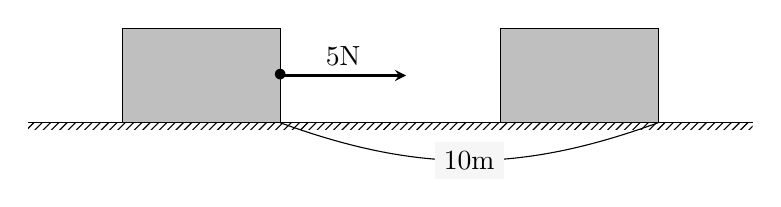
\begin{tikzpicture}[scale = 0.4]
        \path[draw](-3,0) to (20,0);
        \coordinate(A) at (0,0);
        \coordinate(B) at (5,3);
        \coordinate(C) at (12,0);
        \coordinate(D) at (17,3);
        \coordinate(E) at (5,0);
        \coordinate(F) at (17,0);
        
        % rectangle start
        \path[draw, fill = lightgray] (A) rectangle(B);
        % force
        \path[draw, thick, -stealth](5,1.5)node{$\bullet$}to node[midway, above] {5N}(9,1.5);
        % rectangle stop
        \path[draw, fill = lightgray] (C) rectangle(D);
        % distance
        \path[draw](E)to[bend right=20]node[fill=nomesihana!4!white,midway] {10m}(F);
        % resistance
        \path[pattern=north east lines](-3,-0.2)rectangle(20,0);
        \end{tikzpicture}
    \end{center}
    \ref{力の図示} 節の$(\ast)$に注意しながら, 物体にはたらく力を書いていきます. 
    \begin{center}
    \begin{tabular}{cc}
    \begin{minipage}{6cm}
    \begin{tikzpicture}[scale = 0.4]
        % vector
        \coordinate(V1)at(1,0);
        \coordinate(V2)at(0,1);
        % points
        \path[draw](-3,0) to (10,0);
        \coordinate(A) at (0,0);
        \coordinate(B) at (5,3);
        \coordinate(C) at (2,0);
        \coordinate(G) at ($(A)!0.5!(B)$);
        % rectangle start
        \path[draw, fill = lightgray] (A) rectangle(B);
        % force
        \path[draw, thick, -stealth](5,1.5)node{$\bullet$}to node[midway, above] {5N}(8,1.5);
        % gravity
        \path[draw, thick, -stealth](G)node{$\bullet$}to($(G)-4*(V2)$)node[right]{重力};
        % resistance
        \path[draw, thick, -stealth](C)node{$\bullet$}to ($(C)-3*(V1)$)node[below]{摩擦力};
        % 垂直抗力と作用, 反作用
        \path[draw, thick, -stealth](C)to ($(C)+4*(V2)$)node[above]{垂直抗力};
        \path[draw, dashed, -stealth](C)to ($(C)-4*(V2)$)node[below]{$F$};
    \end{tikzpicture}
    \end{minipage}&
    \begin{minipage}{6cm}
    物体にはたらく力の大きさは, 
    \begin{itemize}
        \item 重力：100N
        \item 垂直抗力：100N
        \item 手が物体を引く力：5N
        \item (動)摩擦力：5N (等速で動いているため, 物体にはたらく力はつり合っているはずです.)
    \end{itemize}
    \end{minipage}
    \end{tabular}
    \end{center}
    順に, これらの力が物体に行った仕事を計算してみます. 点線で書いた$F$は, 物体が床を押す力で, 床にかかるため今回は関係ありません. 
    \begin{itemize}
        \item 重力：力の向きは鉛直下向きで, 物体はその方向に動いていない(0m動いた)ため0J.
        \item 垂直抗力：力の向きは, 面に垂直な向きで, 運動の間物体はその方向には動いていない(0m動いた)ため0J.
        \item 手が物体を引く力：5Nでその方向に10m動かしたから, $5\cdot 10 = 50$ [J]
        \item (動)摩擦力：5Nでその方向とは反対向きに10m動かしたから, $5\cdot (-10) = -50$ [J]. 尚, 大きさは50Jです. 
    \end{itemize}
\end{exbox}
また, 仕事に関しては次のような事実が知られており, 直感的にも納得できると思います.
\begin{freebox}{仕事の原理}
    (道具の質量を無視できたり、摩擦がない場合)仕事は道具に依らない.
\end{freebox}
つまり, 同じ仕事をするのに, 別の道具を使っても問題ないということです\footnote{余談ですが, 普段我々が使う「仕事」において成り立つかは微妙です. 例えば, 「物理の資料を作る」という仕事でも, パソコン(OS)によって使えるフォントが違ったり, 印刷機(インクジェットかレーザーか)によって印刷の品質が異なります.}. 
 
重力加速度を10m/s$^2$として, 次のような例を考えてみましょう. 
\begin{exbox}{仕事の原理の例}
   水平面に置かれた質量10kgの物体を, ゆっくり垂直に3m持ち上げるとき, 手で持ち上げる場合と, 軽い定滑車, 軽い動滑車を使って持ち上げる場合を考えます.
   \begin{center}
    \begin{tabular}{ccc}
    手を使う場合 & 定滑車を使う場合 & 動滑車を使う場合\\
    \begin{minipage}{4cm}
    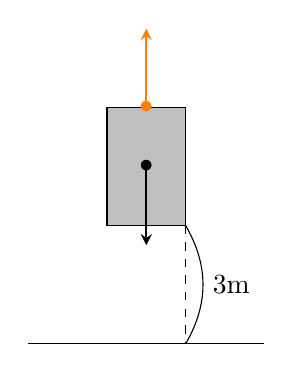
\begin{tikzpicture}[scale = 0.5]
    % ground
    \path[draw](-3,-3)to(3,-3);
    % vector
    \coordinate(V)at(0,1); 
    % point
    \coordinate(O)at(0,0);
    \coordinate(O')at(-1,0);
    \coordinate(P)at(1,3);
    \coordinate(M)at(0,3);
    % bottom
    \coordinate(B)at(1,0);
    % height
    \coordinate(H)at($(B)-3*(V)$);
    \path[draw, dashed](B)to(H);
    \path[draw](B)[bend left=30] to node[midway, right]{3m} (H);
    % gravity
    \coordinate(G)at($(O')!0.5!(P)$);
    \path[draw, fill = lightgray](O')rectangle(P);
    % gravity
    \path[draw, thick, -stealth](G)node{$\bullet$}to($(G)-2*(V)$);
    % pull
    \path[draw, thick, -stealth, orange](M)node{$\bullet$}to($(M)+2*(V)$);
    \end{tikzpicture}
    \end{minipage}&
    \begin{minipage}{4cm}
    \centering
    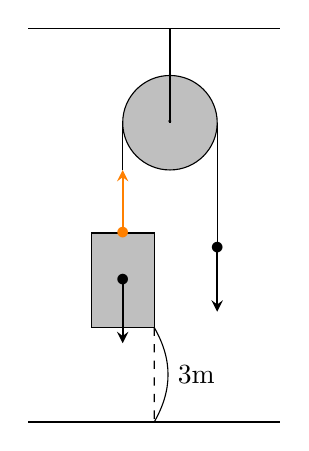
\begin{tikzpicture}[scale = 0.4]
    % ground
    \path[draw](-3,-3)to(5,-3);
    % vector
    \coordinate(V)at(0,1); 
    \coordinate(h)at(1,0);
    % point
    \coordinate(O)at(0,0);
    \coordinate(O')at(-1,0);
    \coordinate(P)at(1,3);
    \coordinate(M)at(0,3);
    % bottom
    \coordinate(B)at(1,0);
    % height
    \coordinate(H)at($(B)-3*(V)$);
    \path[draw, dashed](B)to(H);
    \path[draw](B)[bend left=30] to node[midway, right]{3m} (H);
    % gravity
    \coordinate(G)at($(O')!0.5!(P)$);
    \path[draw, fill = lightgray](O')rectangle(P);
    \path[draw, thick, -stealth](G)node{$\bullet$}to($(G)-2*(V)$);
    % pull
    \path[draw, thick, -stealth, orange](M)node{$\bullet$}to($(M)+2*(V)$);
    % 定滑車
    \coordinate(centerr)at($(M)+3.5*(V)$);
    \coordinate(center)at($(centerr)+1.5*(h)$);
    \path[draw, fill = lightgray](center)circle(1.5);
    \draw(center)node{$\cdot$};
    \path[draw]($(M)+2*(V)$)to(centerr);
    \coordinate(end)at($(centerr)+3*(h)$);
    \path[draw]($(end)$)to($(end)-4*(V)$)node{$\bullet$};
    % force
    \path[draw, thick, -stealth]($(end)-4*(V)$)to($(end)-6*(V)$);
    % ceiling
    \path[draw](center)to($(center)+3*(V)$);
    \path[draw](-3,9.5)to(5,9.5);
    \end{tikzpicture}
    \end{minipage}&
    \begin{minipage}{4cm}
    \centering
    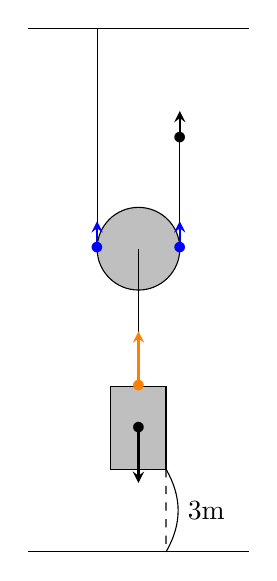
\begin{tikzpicture}[scale = 0.35]
    % vector
    \coordinate(V)at(0,1);
    \coordinate(h)at(1,0);
    % ceiling
    \path[draw](-3,9)to(5,9);
    % point
    \coordinate(M)at(1,9);
    \coordinate(center)at($(M)-8*(V)$);
    \draw(center)node{$\cdot$};
    % line from ceiling
    \path[draw](-0.5,9)to(-0.5,1);
    \path[draw](2.5,1)to(2.5,5);
    % 滑車
    \path[draw, fill = lightgray](center)circle(1.5);
    % pull
    \path[draw, thick, -stealth, blue](-0.5,1)node{$\bullet$}to($(-0.5,1)+(V)$);
    \path[draw, thick, -stealth](2.5,5)node{$\bullet$}to($(2.5,5)+(V)$);
     \path[draw, thick, -stealth, blue](2.5,1)node{$\bullet$}to($(2.5,1)+(V)$);
    % line from 滑車
    \path[draw](center)to($(center)-6.5*(V)$);
    % ground
    \path[draw](-3,-10)to(5,-10);
    % bottom
    \coordinate(B)at(2,-7);
    % 物体
    \path[draw, fill = lightgray](0,-7)rectangle(2,-4);
    % height
    \coordinate(H)at($(B)-3*(V)$);
    \path[draw, dashed](B)to(H);
    \path[draw](B)[bend left=30] to node[midway, right]{3m} (H);
    % gravity
    \coordinate(G)at($(0,-7)!0.5!(2,-4)$);
    \path[draw, thick, -stealth](G)node{$\bullet$}to($(G)-2*(V)$);
    % pull
    \path[draw, thick, -stealth, orange](1,-4)node{$\bullet$}to($(1,-4)+2*(V)$);
    \end{tikzpicture}   
    \end{minipage}
    \end{tabular}
    \end{center}
    物体にはたらく力は, 手または糸が物体を引く力(オレンジ)と, 重力です. また, 動滑車を使う場合では, 糸を手で引いた結果, 動滑車にかかる力を青で表しています.
    \begin{center}
    \begin{tabular}{cccc}
    \hline
    & 手で引く力の大きさ & 動かした距離 & 仕事 \\ \hline
    手を使う場合 & 100N & 3m & 300J\\ \hline
    定滑車を使う場合 & 100N & 3m & 300J\\ \hline
    動滑車を使う場合 & 50N & \textbf{6m} & 300J\\ \hline
    \end{tabular}
    \end{center}
    \textbf{動滑車の場合, 糸2本でオレンジの力を肩代わりできるため, 手で引く力は, 半分の50Nで大丈夫です. しかし仕事の原理から, 300Jの仕事となることは分かっているため, 動滑車の場合は6m引かなければいけないことが分かります}. 
\end{exbox}
\begin{freebox}{仕事率}
    仕事率とは, 1秒間に行った(または受けた)仕事の大きさをいう. 式で書くと
    \begin{equation}
        \textbf{仕事率[W]} = \frac{\textbf{物体に行った(または物体が受けた)仕事 [J]}}{\textbf{仕事をするのにかかった時間 [s]}} \label{仕事率}
    \end{equation}
    である. 
\end{freebox}
 
例えば, 仕事の原理の例において, 持ち上げるに10秒かかっているなら, $300/10 = 30$ [W]が仕事率です. 

ところで仕事率の単位は, 上述の通り[W]となっています. これはなぜでしょうか. 物理で, $\text{[J]} = \text{[W]} \cdot \text{[s]}$となっていることを習ったと思います. 今回, [J]を秒数[s]で割ったため, [W]が登場するわけです. 
\subsection{保存力}\label{保存力}
ここで, 仕事とその経路の関係によって, 力を分類することができるため紹介します.  
\begin{freebox}{保存力}
\textbf{その力がする仕事が経路に依らないとき, その力を保存力という}. 保存力は, 物体の位置変化だけで仕事が決まるような力と言い換えられる.
\end{freebox}
この定義だけでの理解は難しいでしょう. 例により比較してみましょう. 
\begin{exbox}{保存力とそうでない力の例}
あらい斜面上の高さ$h_{1}$の地点から, 高さ$h_{2}$の地点まで, 球が真っ直ぐ滑り降りる場合(経路1)と, 横切って滑り降りる場合(経路2)を考えます. 経路1, 経路2の長さを順に$l_{1}, l_{2}$とします.
\begin{center}
\begin{tabular}{cc}
真横から & 真上から\\
\begin{minipage}{6cm}
\centering
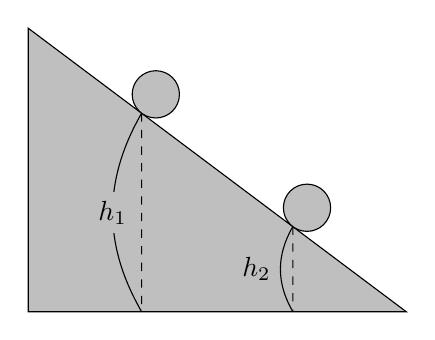
\begin{tikzpicture}[scale = 0.6]
% vector 
\coordinate(v)at(3,4);
\coordinate(O)at(0,0);
\coordinate(A)at(0,6);
\coordinate(B)at(8,0);
\path[draw, fill = lightgray](O)to(A)to(B)to cycle;
% sphere before
\coordinate(c1)at($(A)!0.3!(B)$);
\coordinate(c2)at($(c1)+0.1*(v)$);
\path[draw, fill = lightgray](c2)circle(0.5);
% sphere after
\coordinate(c3)at($(A)!0.7!(B)$);
\coordinate(c4)at($(c3)+0.1*(v)$);
\path[draw, fill = lightgray](c4)circle(0.5);
% vertical line
\coordinate(h1)at($(O)!(c1)!(B)$);
\coordinate(h2)at($(O)!(c3)!(B)$);
\path[draw, dashed](c1)to(h1);
\path[draw, dashed](c3)to(h2);
\path[draw](c1)[bend right = 30] to node[fill = lightgray, midway]{$h_{1}$} (h1);
\path[draw](c3) [bend right = 30] to node[left]{$h_{2}$} (h2);
\end{tikzpicture}
\end{minipage}&
\begin{minipage}{6cm}
\centering
\begin{tikzpicture}[scale = 0.3]
% vector 
\coordinate[label=below:{経路1}](O)at(0,0);
\coordinate(A)at(0,12);
\coordinate[label=below:{経路2}](B)at(5,0);
\path[draw, thick, -stealth](A)to(O);
\path[draw, thick, -stealth](A)to(B);
\path[draw](A)[bend right = 30]to node[fill = nomesihana!4!white, midway]{$l_{1}$} (O);
\path[draw](A)[bend left = 30] to node[fill = nomesihana!4!white, midway]{$l_{2}$} (B);
\end{tikzpicture}
\end{minipage}
\end{tabular}
\end{center}
重力の大きさを$W$ [N]とし, 摩擦力の大きさを$f$ [N]とすると, 
\begin{enumerate}
    \item 重力のした仕事の大きさは, 経路1でも経路2でも, 結果重力の方向に$h_{1} - h_{2}$ [m] だけ動かしたから, $W(h_{1} - h_{2})$ [J]. 
    \item 摩擦力のした仕事の大きさは, 経路1では$fl_{1}$ [J], 経路2では$fl_{2}$ [J]です. しかし$l_{1} < l_{2}$のため, 経路によって仕事の大きさが変わっています. 
\end{enumerate}
よって重力は保存力で, 摩擦力は保存力でないことが分かります. 
\end{exbox} 
 
例えば, 重力(万有引力), ばねの弾性力, 静電気力などは保存力です. 一方, 摩擦力や空気抵抗などは保存力ではありません.
\subsection{エネルギーとは}
普段, エネルギーをいう言葉はよく聞くことでしょう. しかし, 「エネルギーとは何か」と聞かれると案外答えるのが難しいのではないでしょうか. 物理でいうエネルギーとは, 次のようなものです.
\begin{freebox}{エネルギーとは}
物体に仕事を行う能力を, エネルギーという.   
\end{freebox}
\begin{exbox}{エネルギーの例}
    電流を流すことで, モーターを動かすことができたり, 化学変化により, 爆発を起こすことができたりします. これらのエネルギーは順に, 電気エネルギー, 化学エネルギーといいます. 
\end{exbox}
ここからしばらく, 代表的なエネルギーについて紹介, 考察が続きます. 
\subsection{物体の運動エネルギー}
自分が道にボケーッと\footnote{別にボケーッとしていなくても良いけれど}立っているとして, 突進するおすもうさんとぶつかったら, 自分はふっ飛ばされてしまうでしょう. つまり, 私は力を加えられ, 動かされた$\Longleftrightarrow$ 仕事をされたことになります. このように, \textbf{運動する物体は, 他の物体に対して仕事を行う能力があり, それを運動エネルギーといいます}. 運動エネルギーは, 次のような式で与えられることが知られています. 
\begin{freebox}{物体の運動エネルギー}
    速さ$v$ [m/s]を持つ質量$m$ [kg] の物体が持つ運動エネルギーは, 
    \begin{equation}
        \bm{\frac{1}{2}mv^2} \label{運動エネルギー}
    \end{equation}
    で与えられる.
\end{freebox}
\eqref{運動エネルギー} 式を眺めると, 次のようなことが分かるでしょう.
\begin{itemize}
    \item 運動エネルギーは, 質量に比例する.
    \item 運動エネルギーは, 速さの2乗に比例する\footnote{速さが2倍, 3倍, $\cdots$になると, 運動エネルギーは4倍, 9倍$\cdots$になるということ.}.
\end{itemize}
 
直感的には, 重ければ重いほど, 早ければ早いほど相手にダメージを与える事になるということです. また, 速さを変える方が, 質量を変えるよりも, 運動エネルギーに大きな影響を与えやすいということが分かります. 次のような例を考えてみましょう. 
\begin{exbox}{運動エネルギーを考察する}
    壁におすもうさんがぶつかると, 壁は衝撃を受けるはずです.では, 紙飛行機を思い切り投げ, おすもうさんと同じ運動エネルギーをもって壁に衝突させるには, どれくらいの速さが必要でしょうか. 質量$100$ [kg]のおすもうさんが, 5m/sの速さで壁に向かいます. このおすもうさんが持つ運動エネルギーは, $\frac{1}{2}\cdot 100 \cdot 5^2 = 1250$ [J]です. よって, 仮に紙飛行機の質量が0.01 [kg]の場合, 同じだけの運動エネルギーを持たせるには, $1250 = \frac{1}{2} \cdot 0.01 \cdot 500^2$より, 紙飛行機を500 [m/s] で飛ばさなければいけません. ちなみに, 音速は340m/sです.
\end{exbox}
物体の運動エネルギーを理論的に導出してみましょう. 
速度$v_{0}$ [m/s], 質量$m$ [kg]の物体のもつ運動エネルギーを導出しましょう. そこで\textbf{私が}, 速度$v_{0}$ [m/s], 質量$m$ [kg]の物体に一定の力$F$ [N]を加え続けて, $t$秒間でその物体を静止させるのに必要な仕事の大きさを考えます. 物体の運動方程式は, 初速度の向きを正とすると, $-F = ma$であり, $a = -\frac{F}{m}$と表せます.  $v(t) = 0$となるときを考えると, 
\eqref{速度と位置の関係} 式と, $a = -\frac{F}{m}$より, 
\begin{equation}
   0 - v_{0}^2 = 2\cdot -\frac{F}{m}\cdot x,\quad 即ち,\quad Fx = \frac{1}{2}mv_{0}^2
\end{equation}
となります. この式の左辺は, 「$\text{力}\times \text{距離}$」つまり, 私が物体を止めるまでに, 物体が私にした仕事の大きさを表しています(作用, 反作用の法則より, 私も$F$ [N]の力を受けている). よって, 速さ$v_{0}$ [m/s]で運動する質量$m$ [kg]の物体は, $\frac{1}{2}mv_{0}^2$の仕事をする能力があることが分かります. 
\subsection{物体の位置エネルギー}
唐突ですが, 道で歩いていて, 空から動物のカバが降ってきたら, 私は潰されてしまう, つまり, カバから仕事をされることになるでしょう(どんな世界線なんだ). このように, \textbf{(基準より)高い位置にある物体は, 他の物体に仕事をする能力があり, それを重力による位置エネルギーといいます}. 重力加速度を$g$ [m/s$^2$]として, 式で書くと次のようになります.
\begin{freebox}{物体の重力による位置エネルギー}
    基準点から高さ$h$ [m] にある質量$m$ [kg] の物体の持つ位置エネルギーは
    \begin{equation}
        \bm{mgh} \label{位置エネルギー}
    \end{equation}
    で与えられる.
\end{freebox}
 
\eqref{位置エネルギー} 式を眺めることで, 次のことが分かるでしょう.
\begin{itemize}
    \item 位置エネルギーは質量に比例する.
    \item 位置エネルギーは, 物体の基準からの高さに比例する. 
\end{itemize}
直感的には, 高ければ高いほど, 重ければ重いほど, 相手にダメージを与えることになるということです. 

\eqref{位置エネルギー} 式を理論的に導出してみましょう. 一定の重力$mg$ [N]を受けている物体を, 高さ$h$ [m] の地点から基準点(地面)までゆっくり\footnote{持つ力が重力とつり合うようにするということ}持っていくとき, 私の受ける仕事の大きさは, $mgh$となります. よって, 高さ$h$にある物体は, $mgh$ [J] の仕事を行う能力があります\footnote{一定の$mg$の力で$h$だけ動かす能力があるということです.}. 
\subsection{力学的エネルギー保存則}
\textbf{運動エネルギーと位置エネルギーの和を, 力学的エネルギーといいます}. 力学的エネルギーについては, 次のようなことが知られています. 
\begin{freebox}{力学的エネルギーの保存}
    保存力以外の力が仕事をしないとき, 運動エネルギーと, 位置エネルギーの和, 即ち力学的エネルギーは一定値である. つまり以下が成り立つ, 
    \begin{equation}
        \bm{\frac{1}{2}mv^2} + \bm{mgh} = \textbf{一定値}. 
    \end{equation}
\end{freebox}
この文書では, なぜ力学的エネルギーが一定値になるかの説明はしないことにします. 直感的には次のように捉えられるでしょう.
\begin{itemize}
    \item 速さが増える代わりに, 位置が低くなることで合計を一定に保とうとする. 
    \item 位置が低くなる代わりに, 速さが増えることで合計を一定に保とうとする. 
    \item 速さが減る代わりに, 位置が高くなることで合計を一定に保とうとする. 
    \item 位置が高くなる代わりに, 速さが減ることで合計を一定に保とうとする. 
\end{itemize}
\begin{exbox}{力学的エネルギー保存則の例}
    空気抵抗がないとして, 図のような
    あらい平面と, 両端に滑らかな高さ$h$の曲面が繋がった装置を考えます. 最下点の高さを位置エネルギーの基準とし, 高さ$h$の地点で, 質量$m$ [kg]の球から静かに手を離します.
    \begin{center}
        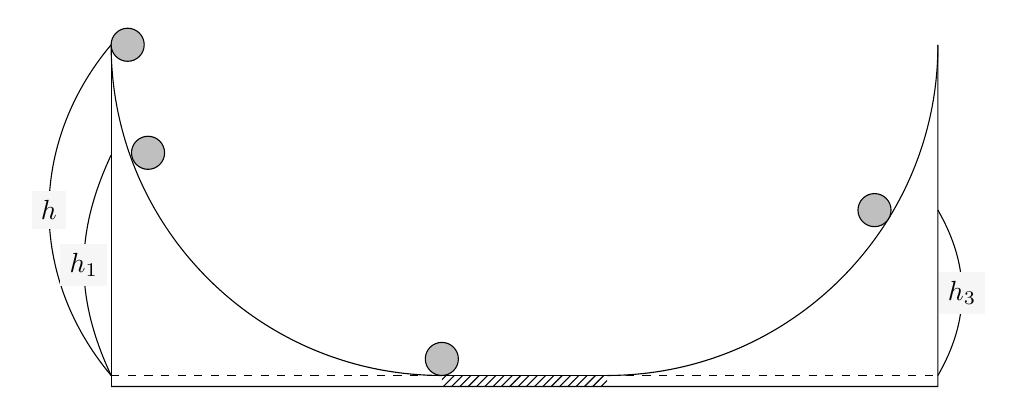
\begin{tikzpicture}[scale = 0.7]
            \coordinate(O)at(0,0);
            \coordinate(O')at(0,-0.2);
            % center of the circle
            \coordinate(P)at(0,6);
            \coordinate(Q)at(9,0);
            \coordinate(Q')at(9,-0.2);
            % path
            \path[draw](O')to(9,-0.2);
            \path[draw](Q')to(15,-0.2)to(15,6);
            \path[draw](6,0)to(Q);
            \path[pattern=north east lines](6,-0.2)rectangle(9,0);
            % arc
            \path[draw](P)arc(180:270:6);
            \path[draw](Q)arc(270:360:6);
            \path[draw](O')to(P);
            % object at h
            \path[draw, fill = lightgray](0.3,6)circle(0.3);
            % object at h1
            \path[draw, fill = lightgray](0.67,4.04)circle(0.3);
            % object at (6,0)
            \path[draw, fill = lightgray](6,0.3)circle(0.3);
            % object at h3
            \path[draw, fill = lightgray](13.85,3)circle(0.3);
            % height
            \path[draw](O)to[bend left=40]node[fill=nomesihana!4!white,, midway] {$h$}(P);
            \path[draw](O)to[bend left=25]node[fill=nomesihana!4!white, midway] {$h_{1}$}(0,4);
            \path[draw](15,3)to[bend left=30]node[fill=nomesihana!4!white, midway] {$h_{3}$}(15,0);
            % base
            \path[draw, dashed](O)to(15,0);
        \end{tikzpicture}
    \end{center}
    \begin{enumerate}
        \item このとき, 力学的エネルギー保存則から
        \begin{itemize}
            \item 高さ$h$ [m]の地点で位置エネルギーが最大, 運動エネルギーが0.
            \item 高さ0 [m]の地点で位置エネルギーが0, 運動エネルギーが最大.
        \end{itemize}
        となることがわかります. 
        \item 球が運動し, 高さ$h_{1}$ [m] ($h_{1} < h$)まで初めて到達した際の速さを求めてみましょう. 求める速さを$v_{1}$ [m/s] とすると, 力学的エネルギーの保存則から, 
        \begin{equation}
            mgh = \frac{1}{2}mv_{1}^2 + mgh_{1}.
        \end{equation}
        これより, $v_{1} = \sqrt{2g(h - h_{1})}$ [m/s]を得ます. つまり, $h_{1}$が小さい$\Longleftrightarrow$ 位置が低くなるほど, 球の速さが大きくなることが式からも分かります. 
        \item 最下点に到達した瞬間の速さを求めてみましょう. 求める速さを$v_{2}$ [m/s]とすると, 力学的エネルギーの保存則から, 
        \begin{equation}
            mgh = \frac{1}{2}mv_{2}^2.
        \end{equation}
        これより$v_{2} = \sqrt{2gh}$ [m/s]となります. (1)で$h_{1} = 0$としたものになっており, このとき速さが最大となることが分かります. 
        \item あらい斜面を通った後, 球が上がることのできる最高地点の高さを$h_{3}$ [m]とします. このとき$h_{3}$は何mでしょうか. 
        
        摩擦に逆らって進むことにエネルギーを使ってしまうため, \textbf{摩擦力のする仕事の分が力学的エネルギーの減少として現れます}. 摩擦力のした仕事の大きさを$E$としましょう. このとき, 力学的エネルギーが, 最初より$E$ [J]だけ減る, 即ち$mgh-E$ [J] となることに注意すると, 減少後の力学的エネルギーの保存則から
        \begin{equation}
            mgh-E = mgh_{3}.\quad h_{3}= h - \frac{E}{mg} \ \text{[m]} \label{temp_力学的エネルギーの保存}
        \end{equation}
        となります. \textbf{つまり, あらい斜面を挟めば, 到達できる高さが$h$よりも減ってしまう}わけです. 
        \item 物体が$h$ [m]の地点から$h_{3}$ [m]の地点に到達するまでに, 垂直抗力が物体にした仕事の大きさは何Jとなるでしょう. 
        
        垂直抗力は, 面に垂直な方向にはたらきますが, 一連の運動で, 面に垂直な方向に物体は動いていないため, 垂直抗力が物体にした仕事の大きさは0[J]です.
    \end{enumerate}
\end{exbox}
高校では, 摩擦係数($\mu$で表されることが多い)を用いることで, 摩擦力が「
$\mu \times 垂直抗力の大きさ$」で表されることを学びます. よって, 水平面の長さを$x$ [m]とすれば, \eqref{temp_力学的エネルギーの保存} 式から
\begin{equation}
    mgh-\mu mgx = mgh_{3}.\quad h_{3}= h - \mu x \ \text{[m]}. 
\end{equation}
よって, 先ほどと同様, 上がれる高さは$h$よりも減少する\footnote{以下のことを用いました. 
\begin{itemize}
    \item 水平面で, 物体の受ける重力と垂直抗力がつり合っている. 
    \item 今回摩擦力のした仕事の大きさは, $摩擦力 \times x = \mu mgx$と表される. 
\end{itemize}
}ことが見て取れます. 特に, (あらい)水平面の長さ$x$を, $x = \frac{h}{\mu}$ [m]に設定すれば, 球は水平面の右端で止まってしまうことが分かります.
\section{ばねの弾性と弾性エネルギー}
エネルギーに触れたところで, 少し唐突かもしれませんが, ばねについても考察を深めてみましょう. ばねは, 弾性や弾性力という概念の良い例になっています. 
\subsection{ばねの弾性とフックの法則}
ばねには, 
\begin{itemize}
    \item 伸ばすと縮んで元の長さに戻ろうとする.
    \item 縮めると伸びて元の長さに戻ろうとする.
\end{itemize}
という性質があります. このように, \textbf{変形された物体が元の状態に戻ろうとする性質を弾性といい, その結果現れる力を弾性力といいます}. ばねの弾性力については次の法則が有名です. 
\begin{freebox}{フックの法則}
    ばねの弾性力は, ばねの伸び(縮み)に比例する. すなわち, 自然長からのばねの伸び(縮み)を$x$ [m], ばねに生じる弾性力を$F$ [N]とし, ばねを伸ばす方向を正とすると, 
    \begin{equation}
        \bm{F} = -\bm{kx}\quad (k > 0 \text{ [N/m] は定数で, ばね定数と呼ばれる}) \label{ばねの基本式}
    \end{equation}
    という関係がある. これは向きを含んだ式である. つまり(ばねの)弾性力は変化の方向と反対向きにはたらくということである. 
\end{freebox}
\begin{exbox}{フックの法則の例}
    1Nの力を加えると0.1 [m] 伸びるばねがあり, ばねの自然長は$0.2$ [m]である. このとき, 
    \begin{enumerate}
        \item ばね定数$k$は, 1mばねを伸ばした際に生じる弾性力の大きさを表すため, $k = 10$ [N / m]です. 
        \item ばねの長さが0.5mになったとき, ばねにはたらく弾性力の大きさは, ばねののびが0.3mであることから, (弾性力も1Nの3倍の) 3 [N]となることがわかります. 尚, \eqref{ばねの基本式} 式を用いると,
        \begin{equation}
            F = -10 \cdot 0.3 = -3 \text{[N]}
        \end{equation}
        が得られます. つまりばねが縮む方向に3Nの力がはたらくということです. 
        \item ばねの長さが0.1mになったとき, ばねの伸びは$-0.1$ [m]です. よって\eqref{ばねの基本式} 式を用いると, 
        \begin{equation}
            F = -10 \cdot (-0.1) = 1 \text{[N]}
        \end{equation}
        が得られます. つまりばねが伸びる方向に1Nの力がはたらくということです.
    \end{enumerate}
\end{exbox}
\eqref{ばねの基本式} 式を見て分かるように, ばねののびと, ばねにはたらく弾性力の「大きさ」をグラフにすると, 次のように比例の直線が書けます. 
\begin{freebox}{フックの法則のグラフ}
グラフは弾性力の「大きさ」に着目している.
\centering
\begin{tikzpicture}[scale=0.4]
    % axis
    \coordinate[label=below left:O](O)at(0,0);
    \coordinate[label=right:{ばねの伸び $x$ [m]}](t)at(10,0);
    \coordinate[label=above:{ばねの弾性力の大きさ $F$ [N]}](x)at(0,8);
    \path[draw, -stealth](-1,0)to(t);
    \path[draw, -stealth, name path = X](0,-1)to(x);
    % velocity
    \path[draw, thick]plot[domain = 0:8]({\x}, {\x})node[right]{$F = kx$}to(O);
\end{tikzpicture}
\end{freebox}
これは完全に高校生向けの説明となりますが, 水に物体を沈め, 手を離すと, 浮力により単振動という運動が起こります. このときは水を一種のばねとしてみなすことができます. 
\subsection{ばねの弾性エネルギー}
$x$ [m]だけ伸びた(縮んだ)ばねは, 物体にどれだけの仕事を行えるでしょうか. つまり, ばねが$x$ [m]だけ伸びた(縮んだ)際に, ばねの持つエネルギーはどのように表せるでしょうか. 例のごとく(？)ばねの弾性力の「大きさ」と伸びのグラフについて, グラフと軸に囲まれた面積を考察してみましょう. 
\begin{center}
\begin{tabular}{cc}
    長方形に分割 & 長方形の分割を細かくする\\
    \begin{minipage}{7cm}
    \begin{center}
    \begin{tikzpicture}[scale=0.37]
        % axis
        \coordinate[label=below left:O](O)at(0,0);
        \coordinate[label=below left:{ばねののび $x$ [m]}](t)at(10,0);
        \coordinate[label=above:{弾性力の大きさ $F$ [N]}](x)at(0,8);
        \path[draw, -stealth](-1,0)to(t);
        \path[draw, -stealth, name path = X](0,-1)to(x);
        % velocity
        \path[draw, name path=C1]plot[domain = 0:10]({\x}, {0.5*\x})node[right]{$F = kx$};
        % 区分求積
        \foreach \x in {0,1,2,...,8}
        {
            \path[draw, fill = lightgray](\x,0)to(\x,{0.5*\x})to(\x+1,{0.5*\x})to(\x+1,0)--cycle; 
        }  
    \end{tikzpicture}
    \end{center}
    \end{minipage}&
    \begin{minipage}{7cm}
    \begin{center}
    \begin{tikzpicture}[scale=0.37]
        % axis
        \coordinate[label=below left:O](O)at(0,0);
        \coordinate[label=below left:{ばねののび $x$ [m]}](t)at(10,0);
        \coordinate[label=above:{弾性力の大きさ$F$ [N]}](x)at(0,8);
        \path[draw, -stealth](-1,0)to(t);
        \path[draw, -stealth, name path = X](0,-1)to(x);
        % velocity
        \path[draw, name path=C1]plot[domain = 0:10]({\x}, {0.5*\x})node[right]{$F = kx$};
        %区分求積
        \foreach \x in {0,1,2,...,44}
        {
            \path[draw,fill=lightgray]({\x/5},0)to({\x/5},{0.5*(\x/5)})to({(\x+1)/5},{0.5*(\x/5)})to({(\x+1)/5},0)--cycle;
        }
    \end{tikzpicture}
    \end{center}
    \end{minipage}
    \end{tabular}
\end{center}
一つ一つの長方形の面積は, $「弾性力の大きさ」\times「伸ばしたばねの長さ」$を表しているため,区切った区間で, ばねが物体に行う仕事の大きさを表すはずです. よって, \textbf{この長方形の面積和は, ばねが$x$だけ伸びる間に, ばねが物体に行う仕事の大きさを表している}ことが分かります. よって, 長方形の分割を限りなく小さくすれば, その面積の和は正確な仕事の大きさを表すことになるでしょう. つまり, \textbf{グラフと伸びの軸で囲まれた部分の面積を求めれば, ばねが$x$だけ伸びる間に, ばねが物体に行う仕事を求めることができるということです}. ばねが$x$[m]伸びるとき, 底辺$x$, 高さ$kx$の三角形の面積を考えることにより, 次が分かります.
\begin{freebox}{ばねの弾性エネルギー}
ばねを変化させた際に. ばねが持つエネルギーを\textbf{ばねの弾性エネルギー}という. ばね定数$k$ [N/m]であるばねの弾性エネルギーの大きさは, そのばねを自然長から$x$ [m]だけ変化させたとき, 
\begin{equation}
    \bm{\frac{1}{2}kx^2}\label{ばねの弾性エネルギー}
\end{equation}
で与えられる. 単位は[J]である. 尚, 積分を知っているなら$\int_{0}^{x}kxdx$を計算すれば良い.
\end{freebox}
\eqref{ばねの弾性エネルギー} 式から分かるように, ばねの弾性力は保存力\footnote{保存力については\ref{保存力} 節を参照してください.}の一種です. つまり, ばねの伸ばし方(縮ませ方)によらず, 結果ばねをどれだけ伸ばした(縮めた)かによって仕事が決まります. 
\subsection{ばねの弾性エネルギーを含めた保存則}
ばねの弾性力は保存力のため, 力学的エネルギーに, ばねの弾性エネルギーを加えたものを考えても, 保存則が成り立ちます. \textbf{また, ばねの弾性エネルギーを含めて, 力学的エネルギーと呼ぶ場合があります}. 
\begin{exbox}{ばねの弾性エネルギーを含めた力学的エネルギー保存則の例}
    なめらかな水平面に置かれたばね定数$k$ [N/m]の軽いばねがあり, その先端に質量$m$ [kg]の物体を取り付けた.
    \begin{center}
    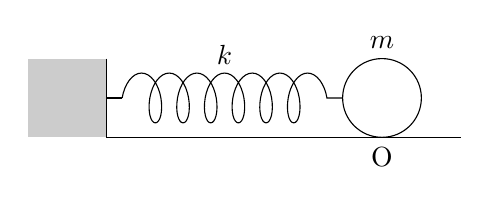
\begin{tikzpicture}
    \fill[black! 20](-4,-0.5) rectangle(-3,0.5);
    \draw (-3,0.5) -- (-3,-0.5);
    \draw (-3,0) -- (-2.8,0);
    \draw (-3,-0.5)--(1.5,-0.5);
    \draw (0.5,-0.5)node[below]{O};
    \draw[decorate,decoration={coil,amplitude=9pt}] (-2.8,0) -- (0,0);
    \draw (-1.5,0.3) node[above] {$k$};
    \draw (0.5,0) circle(0.5);
    \draw (0.5,0.5) node[above]{$m$};
    \end{tikzpicture}
    \end{center}
    \begin{enumerate}
        \item ばねを自然長から$x$ [m]だけのばし, 静かに手を離した. 
        \begin{enumerate}
        \item ばねが自然長に戻る際の物体の速さを求めなさい.
         
        力学的エネルギー保存則から, 自然長に戻る際の速さを$v$ [m/s]とすると, 
        \begin{equation}
            \frac{1}{2}kx^2 = \frac{1}{2}mv^2,\  v = \pm\sqrt{\frac{k}{m}}x.\ v > 0より,\ v = \sqrt{\frac{k}{m}}x \ \text{[m/s]}.
        \end{equation}
        \item ばねが縮みきった際, ばねは自然長から何m縮むことになるか. 
        
        力学的エネルギー保存則から, 縮みきったときの自然長からの縮みを$y$ [m]とすると,
        \begin{equation}
            \frac{1}{2}ky^2 = \frac{1}{2}kx^2,\  y = \pm x.\ よって, x \text{[m]}だけ縮む. 
        \end{equation}
        \end{enumerate}
        \item 次のように, ばねの乗った水平面になめらかな高さ$h$ [m] の斜面を接続した.
        \begin{center}
        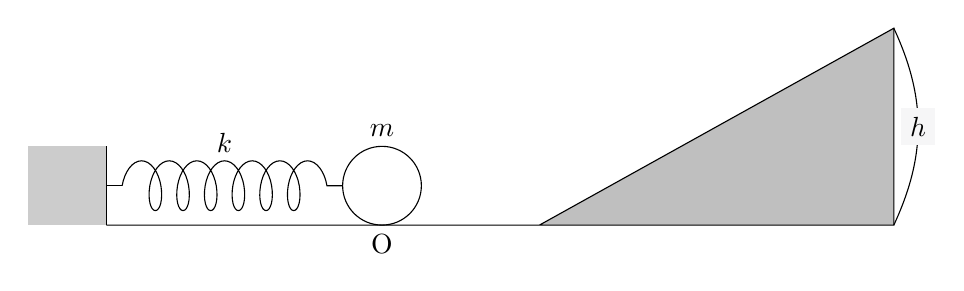
\begin{tikzpicture}
        \fill[black! 20](-4,-0.5) rectangle(-3,0.5);
        \draw (-3,0.5) -- (-3,-0.5);
        \draw (-3,0) -- (-2.8,0);
        \path[draw, fill = lightgray](-3,-0.5)to(2.5,-0.5)to(7,2)to(7,-0.5) to (1.5, -0.5);
        \draw (0.5,-0.5)node[below]{O};
        \draw[decorate,decoration={coil,amplitude=9pt}] (-2.8,0) -- (0,0);
        \draw (-1.5,0.3) node[above] {$k$};
        \draw (0.5,0) circle(0.5);
        \draw (0.5,0.5) node[above]{$m$};
        \path[draw](7,-0.5)to[bend right=25]node[fill=nomesihana!4!white, midway] {$h$}(7,2);
        \end{tikzpicture}
        \end{center}
        ばねを自然長から$x$ [m]だけ縮ませてから, 静かに手を離した. 
        \begin{enumerate}
            \item 運動の途中で物体がばねを離れ, 斜面の中点に到達するとき, その地点での物体の速さを求めなさい. 
            
            求める速さを$v_{M}$とする. 中点は高さ$h/2$ [m]の地点となるから, 力学的エネルギー保存則より
            \begin{equation}
                \frac{1}{2}kx^2 = \frac{1}{2}mv_{M}^2 + mg\cdot \left(\frac{h}{2}\right).\ よって,\ v_{M} = \pm\sqrt{\frac{1}{m}(kx^2-mgh)}.
            \end{equation}
            $v_{M} > 0$より, $\displaystyle v_{M} = \sqrt{\frac{1}{m}(kx^2-mgh)}$ [m/s].\medskip
            \item ばねの縮みが小さいと, 物体の速度が足りず, 高さ$h$の地点に到達できないことが予想される. 高さ$h$の地点まで物体が到達するには, ばねの縮み$x$の値をどのような範囲で設定すれば良いか. 
            
            高さ$h$における運動エネルギーが0 [J]以上あれば良い. よって, 
            \begin{equation}
                \frac{1}{2}kx^2 - mgh\geq 0. \ よって,\ x^2 \geq  \frac{2mgh}{k}.
            \end{equation}
            $x > 0$より$x \geq \sqrt{\dfrac{2mgh}{k}}$となるように縮めないといけない.
        \end{enumerate}
    \end{enumerate}
\end{exbox}
尚, 上の例題の(1)に対して, \ref{一定の力がはたらく運動} 節の\eqref{等加速度直線運動-速度} 式, \eqref{等加速度直線運動-位置} 式や, \eqref{速度と位置の関係} 式を適用できないかと考えた人もいると思います. しかしながら今回, それらの式を使用することはできません. なぜなら, \eqref{ばねの基本式} 式を見て分かるように, ばねの伸びによって弾性力の大きさが変わる, すなわち, 運動中に物体にはたらく力が一定とならないからです. 

\section{浮力と水圧}
この節では, 水圧と浮力に関して考察を深めます. 浮力に関するアルキメデスの原理というものを誓いすることが目標です. 
\subsection{そもそも圧力とは}
圧力という言葉は聞いたことがあると思いますが, それが何かを言語化するの案外難しいのではないでしょうか. 
\begin{freebox}{圧力の定義}
    物体にはたらく圧力とは, 物体のある面に着目したとき, その面の1m$^2$あたりにはたらく力の大きさのことをいう. 単位は [Pa] (パスカル)で, 式にすると次のようになる.
    \begin{equation}
        \textbf{圧力 [Pa]} = \frac{\textbf{その面に対して垂直にはたらく力の大きさ[N]}}{\textbf{その面の面積[m$^2$]}}. \label{圧力の定義式}
    \end{equation}
\end{freebox}
圧力といいながら, 概念としては力と異なることに注意しましょう. 
\begin{exbox}{力と圧力}
    重さが25N, 底面積が0.0625 m$^2$ の物体が水平面に置いてあるとすると, 物体の底面の受ける圧力は, $25/0.0625 = 400$ [Pa]となります. これは, 物体の底面1m$^2$あたりに, 400Nの力を受けているということを表します. 
\end{exbox} 
\subsection{水圧について}
水圧という言葉は聞いたことがあると思います. ここで, 海に潜った場合と, プール(淡水)で潜った場合を考えてみましょう. 実際に潜ってみると, 次のような事がわかると思います. 
\begin{itemize}
    \item 深いほど強い圧がかかる. 
    \item 淡水よりも海水中を潜ったほうが強い圧がかかる.
\end{itemize}
つまり水圧には, 流体の密度と, 水深が関係していることが予想できます. 実際, 水圧を式で表すと次のような形になります. 尚, 大気圧は考えず, 流体からの圧力のみに着目しています.
\begin{freebox}{水圧(流体による圧力)}
    流体(水)中の物体の面には, 流体(水)によりあらゆる方向から圧力が生じ, 流体が水の場合, これを特に\textbf{水圧}という. 流体(水)の密度を$\rho$ [kg/m$^3$], その面の流体中の深さを$h$ [m], その面が受ける圧力の大きさ [Pa] は, 
    \begin{equation}
        \bm{\rho  hg} \label{水圧の式}
    \end{equation}
    で与えられる. $g$ [m/s$^2$]は重力加速度である. 
\end{freebox}
尚, \textbf{水や油, 空気などの流動性のある物体を流体といいます}. \eqref{水圧の式} 式より, 流体による圧力は, 流体中の深さと物体の密度の両方に比例することが分かります. 
\begin{exbox}{水圧の例}
    \begin{itemize}
        \item 例えば水深10mでの水圧が500Paなら, 水深30mでは3倍の1500Paになります. 
        \item 水の入ったペットボトルに穴を開けると, ペットボトルの下にある穴ほど, 飛び出す水の勢いが強いです.
    \end{itemize}
\end{exbox}
それでは\eqref{水圧の式} 式を導出してみましょう. 密度$\rho$ [kg/m$^3$] の流体の深さ$h$ [m]の地点にある物体の面(面積$S$ [m$^2$])を考えてみます. 
\begin{center}
\begin{tabular}{cc}
\begin{minipage}{5cm}
\centering
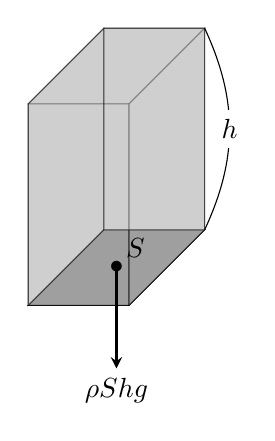
\begin{tikzpicture}[scale=0.32]
    \coordinate(O)at(0,0);
    \coordinate(x)at(1,0); % vector
    \coordinate(y)at(0,1); % vector
    \coordinate(v)at($(x)+(y)$); % vector
    % 直方体OABC-DEFG
    \coordinate(A)at($4*(x)$);
    \coordinate(C)at($3*(v)$);
    \coordinate(B)at($(A)+(C)$);
    \coordinate(D)at($8*(y)$);
    \coordinate(E)at($(A)+(D)$);
    \coordinate(F)at($(E)+3*(v)$);
    \coordinate(G)at($(D)+3*(v)$);
    \coordinate(M)at($(O)!0.5!(B)$);

    \path[draw, fill = gray](O)to(A)to(B)to(C)to cycle; %底面
    \path[draw, fill = lightgray, opacity=0.5](D)to(E)to(F)to(G)to cycle; % 上面
    \path[draw, fill = lightgray, opacity=0.5](O)to(A)to(E)to(D)to cycle; % 手前の面
    \path[draw, fill = lightgray, opacity=0.5](A)to(B)to(F)to(E)to cycle; % 右側面
    \path[draw, fill = lightgray, opacity=0.5](O)to(C)to(G)to(D)to cycle; % 左側面
    \path[draw, fill = lightgray, opacity=0.5](C)to(B)to(F)to(G)to cycle; % 奥の面
    % force
    \path[draw, thick, -stealth](M)to($(M)-4*(y)$)node[below]{$\rho Shg$};
    \draw(M)node[above right]{$S$};
    \draw(M)node{$\bullet$};
    \path[draw](F)to [bend left=25] node[midway, fill = white]{$h$} (B);
\end{tikzpicture}
\end{minipage}&
\begin{minipage}{8cm}
その面の上には流体が乗っており, その質量は, 流体の密度が$\rho$より, $\rho Sh$[kg] となります. よってその面が流体により受ける力の大きさは, 流体にはたらく重力の大きさを考え, $\rho Shg$ [N]です. 以上から, 流体により面が受ける圧力は, \eqref{圧力の定義式} 式より, 
\begin{equation}
    \frac{\rho Shg}{S} = \rho hg
\end{equation}
となります. 
\end{minipage}
\end{tabular}
\end{center}
\subsection{浮力について}
次に, 流体中にある物体が受ける浮力を説明します. そもそも浮力はなぜ生じるのでしょうか. 鍵となるのは水圧です. 水圧は水深に比例するのでした. よって物体を流体中に沈めたとき, 物体の上面, 下面それぞれが流体から受ける力を考えると,\textbf{物体の下面, つまり水深が深い方が, 上面よりも大きい力を受け, それらの力の差として浮力が生じます. 向きはもちろん鉛直上向きです}.
\begin{center}
\begin{tabular}{cc}
\begin{minipage}{7cm}
\centering
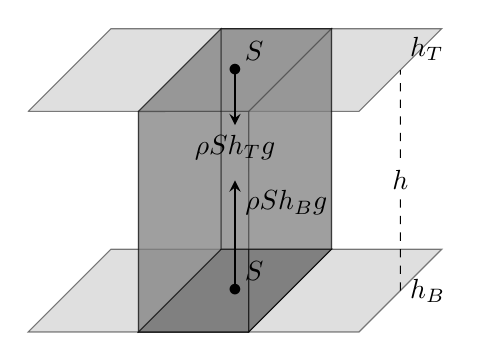
\begin{tikzpicture}[scale=0.35]
    \coordinate(O)at(0,0);
    \coordinate(x)at(1,0); % vector
    \coordinate(y)at(0,1); % vector
    \coordinate(v)at($(x)+(y)$); % vector
    % 直方体OABC-DEFG
    \coordinate(A)at($4*(x)$);
    \coordinate(C)at($3*(v)$);
    \coordinate(B)at($(A)+(C)$);
    \coordinate(D)at($8*(y)$);
    \coordinate(E)at($(A)+(D)$);
    \coordinate(F)at($(E)+3*(v)$);
    \coordinate(G)at($(D)+3*(v)$);
    \coordinate(MB)at($(O)!0.5!(B)$);
    \coordinate(MT)at($(D)!0.5!(F)$);

    % 深さh_Tの面
    \coordinate(D')at($(D)-4*(x)$);
    \coordinate(E')at($(E)+4*(x)$);
    \coordinate(F')at($(F)+4*(x)$);
    \coordinate(G')at($(G)-4*(x)$);
    \path[draw, fill = lightgray, opacity=0.5](D')to(E')to(F')to(G')to cycle;
    \coordinate[label = above right:$h_{T}$](hT)at($(E')!0.5!(F')$);
    
    % 深さh_Bの面
    \coordinate(O')at($(O)-4*(x)$);
    \coordinate(A')at($(A)+4*(x)$);
    \coordinate(B')at($(B)+4*(x)$);
    \coordinate(C')at($(C)-4*(x)$);
    \coordinate[label = right:$h_{B}$](hB)at($(A')!0.5!(B')$);
    \path[draw, fill = lightgray, opacity=0.5](O')to(A')to(B')to(C')to cycle;

    % 高さh
    \path[draw, dashed](hB)to node[midway, fill = white]{$h$} (hT);

    % 物体
    \path[draw, fill = gray](O)to(A)to(B)to(C)to cycle; %底面
    \path[draw, fill = gray, opacity=0.5](D)to(E)to(F)to(G)to cycle; % 上面
    \path[draw, fill = gray, opacity=0.5](O)to(A)to(E)to(D)to cycle; % 手前の面
    \path[draw, fill = gray, opacity=0.5](A)to(B)to(F)to(E)to cycle; % 右側面
    \path[draw, fill = gray, opacity=0.5](O)to(C)to(G)to(D)to cycle; % 左側面
    \path[draw, fill = gray, opacity=0.5](C)to(B)to(F)to(G)to cycle; % 奥の面

    % force bottom
    \path[draw, thick, -stealth](MB)to($(MB)+4*(y)$)node[below right]{$\rho Sh_{B}g$};
    \draw(MB)node[above right]{$S$};
    \draw(MB)node{$\bullet$};

    % force top
    \path[draw, thick, -stealth](MT)to($(MT)-2*(y)$)node[below]{$\rho Sh_{T}g$};
    \draw(MT)node[above right]{$S$};
    \draw(MT)node{$\bullet$};
\end{tikzpicture}
\end{minipage}&
\begin{minipage}{7cm}
上面, 底面の水深がそれぞれ$h_{T}$, $h_{B}$ [m]である, 高さ$h$の直方体の物体にはたらく浮力を考えます. 物体の上面, 下面の面積を$S$ [m$^2$]とし, 流体の密度を$\rho$ [kg/m$^3$] とします. \eqref{水圧の式} 式を思い出しておきましょう.
\end{minipage}
\end{tabular}
\end{center}
\medskip
\begin{center}
\begin{tabular}{cccc}
    \hline
    面 & 面積  [m$^2$]& 流体による圧力 [Pa] & 面が受ける力 [N]\\ \hline
    物体の上面 & $S$ & $\rho h_{T}g$ & $\rho h_{T}gS$ \\ \hline
    物体の下面 & $S$ & $\rho h_{B}g$ & $\rho h_{B}gS$\\
    \hline
\end{tabular}
\end{center}
物体の下面の受ける力のほうが大きいことに注意して, これらの差は
\begin{equation}
    \rho h_{B}gS- \rho h_{T}gS = \rho (h_{B}S - h_{T}S)g = \rho (h_{B} - h_{T})Sg = \rho hSg = \rho V g
\end{equation}
となります\footnote{$hS$が直方体の体積を表していることに注意しましょう. また, 直方体でない形状の場合にも, 発展的な積分をすることで同様の結論を得られます. }.  \textbf{浮力の作用点は, 物体の「流体中にある部分の重心」となります}. 
\begin{freebox}{流体中の物体が受ける浮力}
    物体が密度$\rho$ [kg/m$^3$] の流体に浸かっており, 流体中に入っている部分の体積が$V$ [m$^3$] であるとする. このとき, その物体が流体から受ける浮力の大きさ [N] は, 
    \begin{equation}
        \bm{\rho V g} \label{浮力の式}
    \end{equation}
    で与えられる. $g$ [m/s$^2$] は重力加速度である. \textbf{浮力の作用点のことを浮心という}. 
\end{freebox}
\eqref{浮力の式} 式より, 浮力は, 物体の流体中にある部分の体積に比例します. ここで, $\rho Vg$という式をよく見ると, これは体積$V$ [m$^3$] , 密度$\rho$ [kg/m$^3$] の流体にはたらく重力の大きさ(重さ)を表していることが分かります. よって, 次のようなことがいえます\footnote{アルキメデスという人が発見したため, その名前がついています. 彼は古代ギリシア時代の人物であり, 科学者, 発明家として知られています.}.
\begin{freebox}{浮力に関するアルキメデスの原理}
\textbf{物体が受ける浮力の大きさは, その物体が押しのけた体積の流体の重さに等しい.}
\end{freebox}
これだけでは分かりにくいかと思うため, 例を挙げてみます.
\begin{exbox}{アルキメデスの原理}
\begin{itemize}
\item 重力加速度を10m/s$^2$とします. 密度が2g/cm$^3$の流体に, 体積200cm$^3$の物体を全て沈めた場合を考えます. 
\begin{center}
\begin{tabular}{cc}
\begin{minipage}{5cm}
\centering
\begin{tikzpicture}[scale=0.43]
%水枠
\fill[lightgray](5,0,5)to(5,0,0)to(5,4,0)to(5,4,5)--cycle; %枠右
\fill[lightgray](0,0,5)to(0,0,0)to(0,4,0)to(0,4,5)--cycle; %枠左
\fill[lightgray](0,4,5)to(5,4,5)to(5,4,0)to(0,4,0)--cycle; %枠上
\fill[lightgray](0,0,5)to(5,0,5)to(5,4,5)to(0,4,5)--cycle; %枠手前

%水枠
\draw[gray](5,0,5)to(5,0,0)to(5,4,0)to(5,4,5)--cycle; %枠右
\draw[gray](0,0,5)to(0,0,0)to(0,4,0)to(0,4,5)--cycle; %枠左
\draw[gray](0,4,5)to(5,4,5)to(5,4,0)to(0,4,0)--cycle; %枠上
\draw[gray](0,0,5)to(5,0,5)to(5,4,5)to(0,4,5)--cycle; %枠手前


%大枠
\draw(5,0,5)to(5,0,0)to(5,5,0)to(5,5,5)--cycle; %枠右
\draw(0,0,5)to(0,0,0)to(0,5,0)to(0,5,5)--cycle; %枠左
\draw(0,5,5)to(5,5,5)to(5,5,0)to(0,5,0)--cycle; %枠上
\draw(0,0,5)to(5,0,5)to(5,5,5)to(0,5,5)--cycle; %枠手前
\draw(0,0,5)to(5,0,5)to(5,0,0)to(0,0,0)--cycle; %枠下

\draw(2,4,0)node[right]{流体};

%小枠塗り
\fill[gray](3,0,3)to(3,0,1)to(3,2,1)to(3,2,3)--cycle; %枠右
\fill[gray](1,0,3)to(1,0,1)to(1,2,1)to(1,2,3)--cycle; %枠左
\fill[gray](1,2,3)to(3,2,3)to(3,2,1)to(1,2,1)--cycle; %枠上
\fill[gray](1,0,3)to(3,0,3)to(3,2,3)to(1,2,3)--cycle; %枠手前
\fill[gray](1,0,3)to(3,0,3)to(3,0,1)to(1,0,1)--cycle; %枠下

%小枠
\draw(3,0,3)to(3,0,1)to(3,2,1)to(3,2,3)--cycle; %枠右
\draw(1,0,3)to(1,0,1)to(1,2,1)to(1,2,3)--cycle; %枠左
\draw(1,2,3)to(3,2,3)to(3,2,1)to(1,2,1)--cycle; %枠上
\draw(1,0,3)to(3,0,3)to(3,2,3)to(1,2,3)--cycle; %枠手前
\draw(1,0,3)to(3,0,3)to(3,0,1)to(1,0,1)--cycle; %枠下
\end{tikzpicture}
\end{minipage}
&
\begin{minipage}{5cm}
この体積の流体を押しのけている.\\\\
\centering
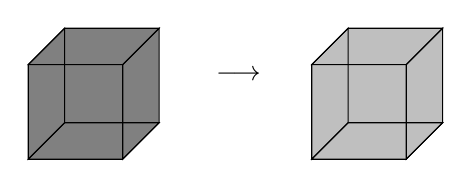
\begin{tikzpicture}[scale=0.6]
%物体小枠塗り
\fill[gray](2,0,2)to(2,0,0)to(2,2,0)to(2,2,2)--cycle; %枠右
\fill[gray](0,0,2)to(0,0,0)to(0,2,0)to(0,2,2)--cycle; %枠左
\fill[gray](0,2,2)to(2,2,2)to(2,2,0)to(0,2,0)--cycle; %枠上
\fill[gray](0,0,2)to(2,0,2)to(2,2,2)to(0,2,2)--cycle; %枠手前

%物体小枠
\draw(2,0,2)to(2,0,0)to(2,2,0)to(2,2,2)--cycle; %枠右
\draw(0,0,2)to(0,0,0)to(0,2,0)to(0,2,2)--cycle; %枠左
\draw(0,2,2)to(2,2,2)to(2,2,0)to(0,2,0)--cycle; %枠上
\draw(0,0,2)to(2,0,2)to(2,2,2)to(0,2,2)--cycle; %枠手前
\draw(0,0,2)to(2,0,2)to(2,0,0)to(0,0,0)--cycle; %枠下

\draw(3,1,0)node[right]{$\longrightarrow$};

%小枠塗り
\fill[lightgray](8,0,2)to(8,0,0)to(8,2,0)to(8,2,2)--cycle; %枠右
\fill[lightgray](6,0,2)to(6,0,0)to(6,2,0)to(6,2,2)--cycle; %枠左
\fill[lightgray](6,2,2)to(8,2,2)to(8,2,0)to(6,2,0)--cycle; %枠上
\fill[lightgray](6,0,2)to(8,0,2)to(8,2,2)to(6,2,2)--cycle; %枠手前
\fill[lightgray](6,0,2)to(8,0,2)to(8,0,0)to(6,0,0)--cycle; %枠下

%小枠
\draw(8,0,2)to(8,0,0)to(8,2,0)to(8,2,2)--cycle; %枠右
\draw(6,0,2)to(6,0,0)to(6,2,0)to(6,2,2)--cycle; %枠左
\draw(6,2,2)to(8,2,2)to(8,2,0)to(6,2,0)--cycle; %枠上
\draw(6,0,2)to(8,0,2)to(8,2,2)to(6,2,2)--cycle; %枠手前
\draw(6,0,2)to(8,0,2)to(8,0,0)to(6,0,0)--cycle; %枠下
\end{tikzpicture}
\\
\centering
物体(200cm$^3$) \quad 流体(200cm$^3$)
\end{minipage}
\end{tabular}
\end{center}
 
物体が受ける浮力は, 押しのけた流体の質量が$2\text{[g/cm$^3$]} \cdot 200\text{[cm$^3$]}=400$ [g] のため, 4Nとなります.
\item タンカー(貨物船)は, 鉄でできているにも関わらず, 海に浮かび, 重い荷物を多く運ぶことができます. \url{https://illustimage.com/?dl=1012}
\begin{center}
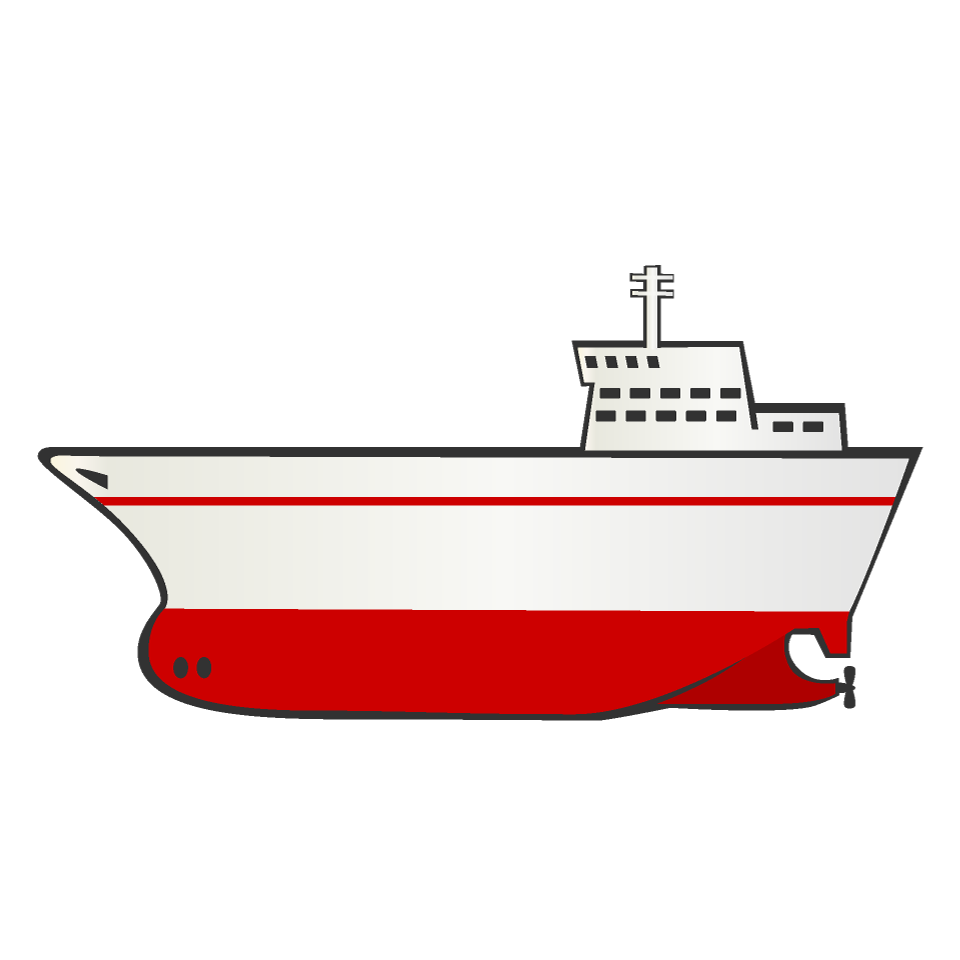
\includegraphics[scale = 0.1]{fig/1012.png}
\end{center}
\vspace{-1cm}
これは, 船底の海水を押しのける部分の体積を大きくすることで, 大きな浮力を受けられるようにし, 更に内部に多くの空間を作ることで, 船体の密度を小さくしているためです. 
\end{itemize}
\end{exbox}

\begin{exbox}{浮力に関するその他の例}
    \begin{itemize}
    \item 「物体の密度が流体の密度よりも大きければ物体は沈んでいき, 小さければ浮き上がってくる」という事実は有名ですが, これを理論的にも導いてみましょう. 物体の密度, 体積それぞれを$\rho_{1}$ [kg/m$^3$] , $V$ [m$^3$] とし, 流体の密度を$\rho_{2}$ [kg/m$^3$] とします.
        
    物体を, 流体中に物体全体が入るように手で支えて(押さえて)おき, 静かに手を離します. このとき, 物体にはたらく重力は$\rho_{1} Vg$ [N], 
    物体にはたらく浮力は$\rho_{2}Vg $ [N] となります. 例えば物体が浮き上がっていくときは, 物体にはたらく浮力が重力よりも大きくなるため, 
    \begin{equation}
        \rho_{2} Vg > \rho {1}Vg,\ すなわち\ \rho_{2} > \rho_{1}.
    \end{equation}
    同様に, 物体が沈んでいくときは, $\rho_{2} < \rho_{1}$となり, 確かに正しいことが確認できます.
    \item 密度$\rho_{1}$ [kg/m$^3$] で, 体積$V$ [m$^3$]の物体の$a$ [％] ($0 < a < 100$)が, 密度$\rho_{2}$ [kg/m$^3$]の流体中に浸かって静止しているとします. このとき, $a$は密度$\rho_{1}$, $\rho_{2}$を用いてどのように表せるでしょうか.
    
    流体中にある物体の体積は$aV$であり, その部分が受ける浮力は$\rho_{2}aVg$です. また, 物体にはたらく重力の大きさは, $\rho_{1}Vg$と表せます. 浮力と重力のつり合いから, 
    \begin{equation}
        \rho_{2}aVg = \rho_{1}Vg.\ よって\ a = \frac{\rho_{1}}{\rho_{2}}.
    \end{equation}
    例えば水に浮いて静止している氷を考えると, 水の密度1000kg/m$^3$, 氷の密度917kg/m$^3$より, $\rho_{1} = 917$, $\rho_{2} = 1000$として, 氷のうち91.7％が水中に浸かっていることが分かるわけです. 
\end{itemize}
\end{exbox}
\section{運動量とその保存}
こちらは完全に高校物理の内容となりますが, 運動量というものにも保存則が成り立つため紹介しようと思います. 保存則の導出の際には作用, 反作用の法則が重要になります. 
\begin{freebox}{運動量}
    速度$v$ [m/s]で運動する質量$m$ [kg]の物体について, $\bm{mv}$\textbf{を運動量という}.
\end{freebox}
運動量はエネルギーと違い, 向きまで扱うことができるという点で柔軟性があります. また, 運動量について, 物体たちにはたらく外力の合力が0である限り, 保存則が成り立ちます.  
\begin{freebox}{運動量保存則}
    質量$m_{1}$ [kg]で速度$v_{1}$ [m/s]の物体1が, 質量$m_{2}$ [kg] で速度$v_{2}$ [m/s]で運動する物体2と衝突したのち, それぞれの速度が$v_{1}'$ [m/s], $v_{2}'$ [m/s]になったとする. このとき, 運動量について以下が成り立つ.
    \begin{equation}
        \bm{m_{1}v_{1}} + \bm{m_{2}v_{2}} = \bm{m_{1}v_{1}'} + \bm{m_{2}v_{2}'}. \label{運動量保存則}
    \end{equation}
    \begin{center}
    \begin{tabular}{ccc}
        \begin{minipage}{3cm}
        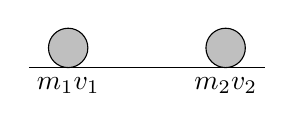
\begin{tikzpicture}[scale = 0.5]
            % ground
            \path[draw](-3,0)to(3,0);
            
            % 衝突前
            % 物体1 
            \coordinate(b1b)at(-2,0.5);
            \coordinate[label=below:{$m_{1}v_{1}$}](b1g)at(-2,0);
            \path[draw, fill = lightgray](b1b)circle(0.5);
            % 物体2 
            \coordinate(b2b)at(2,0.5);
            \coordinate[label=below:{$m_{2}v_{2}$}](b2g)at(2,0);
            \path[draw, fill = lightgray](b2b)circle(0.5);
        \end{tikzpicture}
        \end{minipage}&
        \begin{minipage}{3cm}
        \begin{tikzpicture}[scale = 0.5]
            % ground
            \path[draw](-3,0)to(3,0);
            % 衝突
            % 物体1 
            \coordinate(b1)at(-1,0.5);
            \coordinate(b1g)at(-1,0);
            \path[draw, fill = lightgray](b1)circle(0.5);
            % 物体2 
            \coordinate(b2)at(0,0.5);
            \coordinate(b2g)at(0,0);
            \path[draw, fill = lightgray](b2)circle(0.5);
            \coordinate[label = below:衝突](M)at($(b1g)!0.5!(b2g)$);
        \end{tikzpicture}
        \end{minipage}&
        \begin{minipage}{3cm}
        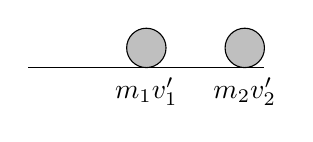
\begin{tikzpicture}[scale = 0.5]
            % ground
            \path[draw](-3,0)to(3,0);
            % 衝突後
            % 物体1 
            \coordinate(b1a)at(0,0.5);
            \coordinate[label=below:{$m_{1}v_{1}'$}](b1g)at(0,0);
            \path[draw, fill = lightgray](b1a)circle(0.5);
            % 物体2 
            \coordinate(b2a)at(2.5,0.5);
            \coordinate[label = below:{$m_{2}v_{2}'$}](b2g)at(2.5,0);
            \path[draw, fill = lightgray](b2a)circle(0.5);
        \end{tikzpicture}           
        \end{minipage}
    \end{tabular}
\end{center}
\end{freebox}
\eqref{運動量保存則} 式が成り立つことを理論的に導出してみましょう. 
まず準備として, 力積という量を定義します. 質量$m$ [kg]の物体に, 時刻$t_{0}$から$t_{1}$ [s]の間, 一定の力$F$ [N]がはたらいて, 物体の速度が$v_{0}$から$v_{1}$ [m/s]まで変化したとしましょう. このとき\eqref{加速度} 式より, $a = \frac{v_{1} - v_{0}}{t_{1} - t_{0}}$です. これを用いて, 物体の運動方程式を書き直すと, 
\begin{equation}
    F = m \cdot \frac{v_1 - v_{0}}{t_{1} - t_{0}}
\end{equation}
となります. 変形して
\begin{equation}
F(t_{1} - t_{0}) = mv_{1} - mv_{0}
\end{equation}となるため, \textbf{左辺は運動量の変化を表していることが分かります}. 
 
\begin{freebox}{力積}
時刻$t_{0}$ [s]から時刻$t_{1}$ [s]の, $\Delta t = t_{1}-t_{0}$ 秒間に, 物体に一定の力$F$ [N] がはたらいたとする. このとき, 
\begin{equation}
    \bm{F\Delta t} \label{力積の式}
\end{equation}
を\textbf{力積}という. また, 上での考察のように, 
\begin{equation}
    \bm{F\Delta t} = \bm{mv_{1}} - \bm{mv_{0}}
\end{equation}
が成り立ち, \textbf{力積は$\bm{\Delta t}$秒間での運動量の変化を表している}. 尚, 力積は向きを含んでいることにも注意せよ.
\end{freebox}
それでは運動量保存則の導出です. 物体1と物体2が接触するとき, (ごく短い)時間$\Delta t$秒間で, 作用, 反作用の法則より, 物体1と物体2は, 大きさが同じ, 向きが反対向きで一直線上にある力$F$を受けます\footnote{$\Delta t$が十分小さいものとし, その間$F$の大きさは一定としています.}. 
\begin{center}
    \begin{tikzpicture}[scale = 0.8]
        % ground
        \path[draw](-3,0)to(3,0);
        % 衝突
        % 物体1 
        \coordinate(b1)at(-0.5,0.5);
        \coordinate(b1g)at(-0.5,0);
        \path[draw, fill = lightgray](b1)circle(0.5);
        % 物体2 
        \coordinate(b2)at(0.5,0.5);
        \coordinate(b2g)at(0.5,0);
        \path[draw, fill = lightgray](b2)circle(0.5);
        \coordinate[label = below:衝突](Mg)at($(b1g)!0.5!(b2g)$);
        \coordinate(M)at($(b1)!0.5!(b2)$);
        % force
        \path[draw, thick, -stealth](M)to(-3, 0.5)node[left]{$F$};
        \path[draw, thick, -stealth](M)to(3, 0.5)node[right]{$-F$};
        \draw(M)node{$\bullet$};
    \end{tikzpicture}
\end{center}
\vspace{-4mm}
よって, 物体それぞれの力積は, 物体1の受ける力の向きを正として, 
\begin{equation}
\begin{cases}
    \text{物体1} & F\Delta t = m_{1}v_{1}' - m_{1}v_{1},\\
    \text{物体2} & -F\Delta t = m_{2}v_{2}' - m_{2}v_{2}.
\end{cases}
\end{equation}
両辺を加えることで, 力積がキャンセルされ, 
\begin{equation}
    0 = m_{1}v_{1}' - m_{1}v_{1} + m_{2}v_{2}' - m_{2}v_{2} \ となり,\quad m_{1}v_{1} + m_{2}v_{2} = m_{1}v_{1}' + m_{2}v_{2}' 
\end{equation}
を得ます. 

次のような例題を考えてみましょう. 
\begin{exbox}{運動量保存則の例題}
滑らかな水平面において, 質量$M$ [kg]で, 速度$v_{1}$で運動していた物体1が, 静止していた質量$m$ [kg]の物体2にぶつかった. 
\begin{center}
    \begin{tabular}{cc}
        \begin{minipage}{6cm}
        \centering
        \begin{tikzpicture}[scale = 0.7]
            % ground
            \path[draw](-3,0)to(3,0);
            % 衝突前
            % 物体1 
            \coordinate(b1b)at(-2,0.5);
            \coordinate[label=below:{物体1}](b1g)at(-2,0);
            \path[draw, fill = lightgray](b1b)circle(0.5);
            % 物体2 
            \coordinate(b2b)at(2,0.5);
            \coordinate[label=below:{物体2}](b2g)at(2,0);
            \path[draw, fill = lightgray](b2b)circle(0.5);
        \end{tikzpicture}
        \end{minipage}&
        \begin{minipage}{6cm}
        \centering
        \begin{tikzpicture}[scale = 0.7]
            % ground
            \path[draw](-3,0)to(3,0);
            % 衝突
            % 物体1 
            \coordinate(b1)at(-1,0.5);
            \coordinate(b1g)at(-1,0);
            \path[draw, fill = lightgray](b1)circle(0.5);
            % 物体2 
            \coordinate(b2)at(0,0.5);
            \coordinate(b2g)at(0,0);
            \path[draw, fill = lightgray](b2)circle(0.5);
            \coordinate[label = below:衝突](M)at($(b1g)!0.5!(b2g)$);
        \end{tikzpicture}
    \end{minipage}
    \end{tabular}
\end{center}
\begin{enumerate}
    \item 衝突直後, 滑らかな水平面上を2つの物体が一体となって運動し始めたとするとき, 2つの物体の速度を求めなさい.
    
    一体になったため, 速度が同じになる. 運動量保存則から, 同じ速度になったときの速度を$v$とすると,
    \begin{equation}
        Mv_{1} + 0 = Mv + mv.\quad よって, \quad v = \frac{M}{M+m}v_{1}\ \text{[m/s]}.
    \end{equation}
    \item 衝突直後, 物体1と物体2が一体となって, 動摩擦係数が$\mu$の水平面に突入したとする. それぞれの物体が, 止まるまでに進む距離を求めなさい. 
    
    (1)より, あらい水平面に突入する際の初速度は$\frac{M}{M+m}v_{1}$ [m/s]です. 作用, 反作用の法則による力を$F$ [N]とします.
    \begin{itemize}
    \item 物体1について運動方程式を立てると, 
    \begin{itemize}
        \item 鉛直方向：$Mg - N_{1} = 0$. $N_{1}$は物体1の受ける垂直抗力.
        \item 水平方向：$-\mu N_{1} - F= Ma$. 進行方向を正とした.
    \end{itemize}
    \item 物体2について運動方程式を立てると, 
    \begin{itemize}
        \item 鉛直方向：$mg - N_{2} = 0$. $N_{2}$は物体2の受ける垂直抗力.
        \item 水平方向：$-\mu N_{2} + F= ma$. 進行方向を正とした.
    \end{itemize}
    \end{itemize}
    水平方向についての運動方程式を足し合わせれば$a = -\mu g$を得ます. 尚, 2つを質量$M + m$ [kg]の１つの物体と見なして運動方程式を立てれば同様の結論を得られます. 停止するときは速度が0になるため, \eqref{速度と位置の関係} 式より, 停止するまでに進む距離を$x$ [m]とすると(2つとも同じ距離だけ進みます),
    \begin{equation}
    0^2 - \left(\frac{M}{M+m}v_{1}\right)^2 = 2\cdot (-\mu g)x.\quad x = \frac{M^2v_{1}^2}{2\mu(M+m)^2g}\ \text{[m]}.
    \end{equation}
    \item 衝突直後, 物体1は停止し, 物体2のみが運動し始めたとき, 物体2の速度と, 運動エネルギーを計算しなさい.
    
    運動量保存則から, 物体2が運動しているときの速度を$v'$とすると,
    \begin{equation}
        Mv_{1} + 0 = 0+ mv'.\quad よって, \quad v' = \frac{M}{m}v_{1}\ \text{[m/s]}.
    \end{equation}
    よって, 物体2の持つ運動エネルギーは, 
    \begin{equation}
        \frac{1}{2}\cdot m \left(\frac{M}{m}v_{1}\right)^2 = \frac{M^2}{2m}v_{1}^2\ \text{[J]}.
    \end{equation}
    \item (3)ののち, 滑らかな斜面を物体2が上がっていったとすると, 物体2は何mの高さまで上がることができるか.
    
    力学的エネルギーの保存から, 最高点$h$ [m]での速さが0になると考えて, 
    \begin{equation}
        \frac{M^2}{2m}v_{1}^2 = mgh.\quad h = \frac{M^2v_{1}^2}{2m^2g}\ \text{[m]}.
    \end{equation}
\end{enumerate}
\end{exbox}
\section{ちょっとしたテクニック}
今後, 問題を解いた際に, 解答が複雑になることが増えてくるでしょう. そのときに意識すると良いこととして, 次のようなアドバイスをしておきます.
\begin{itemize}
    \item \textbf{単位を考える}：
    例えば, 直前の例題の(2)では, 距離を聞かれているため, 答えの単位は[m] \medbreak
    となるはずです. $\dfrac{M^2v_{1}^2}{2\mu (M+m)^2g}$について, 単位を確認すると, $\dfrac{\text{[kg]}^2\text{[m/s]}^2}{\text{[kg]}^2\cdot \text{[m/s$^2$]}}$. [kg]$^2$がキャ\medbreak
    ンセルされ, $\dfrac{\text{[m/s]}^2}{\text{[m/s$^2$]}} = \dfrac{\text{[m]}^2}{\text{[s]}^2} \div \dfrac{\text{[m]}}{\text{[s]}^2} = \text{[m]}$ となるため, 正しそうだと考えられます.\medskip
    \item \textbf{符号(向き)を考える}：例えば, $M > m > 0$ [kg], $v > 0$ [m/s] のときに, 物体の速度が\medbreak
    $\dfrac{M}{m-M}v$ [m/s]で与えられたとします. $m-M < 0$のため, この速度は負です. よって, \medbreak
    「物体の速さを答えよ」と言われた際には$\dfrac{M}{M-m}v$ [m/s]となります.
\end{itemize}
\end{document}